%\chapter{Introduction}
%\label{chap:intro}

\section{Introduction in english}

\subsection{Data Analysis and Machine Learning}

%\paragraph*{Data Analysis and Machine Learning.} 
Data collection and generation in various human activities, including both industry and academia, have grown 
exponentially over the last decade and are now ubiquitous in many different fields of science, finance and industry.
For example, in digital science, the fast development of image acquisition and processing has allowed large amounts of images to 
become publicly available online~\cite{Lecun98, Krizhevsky09, Nene96, Ojala02, Russell08}.
Similarly, in biology, next generation high-throughput sequencing allowed most laboratories 
to easily determine DNA sequences of sample organisms~\cite{Bindewald06,Goodwin16,Kim16,Metzker10}.  
Hence, the need to summarize and extract useful information from these massive amounts of data has become a problem of primary interest.

Machine Learning is a field of data science that aims at deriving algorithms ("Machine") that can make
predictions about new data solely from the information that is contained in already collected datasets ("Learning").
These techniques can provide answers to multiple data analysis problems such as {\em classification}, which aims at predicting labels,
{\em clustering}, which aims at separating data into groups or clusters, or {\em regression}, which aims at approximating functions on data.
We refer the interested reader to~\cite{Friedman01} for a comprehensive introduction to these methods.
%often called {\em training} datasets.
%The term "Learning" comes from the fact that predictions depend on the training datasets.   
For example, a typical classification problem would be to predict if a drug have effects on a specific patient $P$. This is a binary classification
problem since the label we want to predict for $P$ is either "effect" or "no effects".
Assuming you have a database of patients at hand, in which the drug effects on each patient were recorded, one of the simplest way to proceed is
to look for the closest match, or most similar patient, to $P$ in this database, 
and to take the label of this match.  
This extremely simple yet powerful method
is called {\em nearest neighbor} prediction, and has been extensively studied by data scientists. 
More generally, nearest neighbor prediction is nothing but a small part of the large variety of methods proposed in Machine Learning, 
which can tackle many real-life challenges including image classification, musical genre prediction or medical prognosis to name a few.
More examples of applications and datasets can be found in~\cite{Friedman01}. %on \url{https://en.wikipedia.org/wiki/List_of_datasets_for_machine_learning_research}}.
    


\paragraph*{Descriptors.} Usually, data comes in the form of a point cloud in $\R^D$, where $D\in\N^*$. 
Each data point represents an {\em observation} and each dimension, 
or coordinate, represents a {\em measurement}. For instance, observations can be patients, images or DNA sequences, whose corresponding measurements are
physical characteristics (height, weight, age...), grey scale values of pixels or nucleobases A,C,T,G composing DNA.
It is often the case that the number of measurements is very large, leading to a rich level of information, but also making 
data very high-dimensional and impossible to visualize.  

Hence, a large part of data analysis is devoted to the summarization 
of the information contained in datasets or data points into simple and 
interpretable {\em descriptors} or {\em signatures}, which are usually application specific. 
For instance, among common descriptors are: 
bag-of-words models~\cite{Soumya14} for text document data,
SIFT~\cite{Lowe04} and HoG~\cite{Dalal05} descriptors for image data,
curvature and spin images~\cite{Johnson99} for 3D shape data,
wavelet descriptors~\cite{Mallat08} for signal data,
and, more generally, outputs of data reduction technique, such as MDS, PCA or Isomap~\cite{Tenenbaum00}.
The efficiency of descriptors is very often correlated to the properties they enjoy. Depending on the application,
one may want descriptors  to be translation or rotation invariant, intrinsic or extrinsic, to lie in Euclidean space, etc.
Deriving descriptors with desirable properties is important since it greatly enhances interpretation and visualization, as mentioned above,
but it also improves the performances of Machine Learning algorithms, which may perform poorly if fed with raw data.
The aim of this thesis is to study a specific class of descriptors called {\em topological} descriptors, which are known to be 
%{\em stable}, in the sense that descriptors of similar data cannot be far from each other, and 
invariant to continuous deformations of data that do not involve tearing or gluing~\cite{Carlsson09a}. 

\subsection{Topological Descriptors}

The idea of topological descriptors is to summarize the {\em topological information} contained in data~\cite{Carlsson09a}.
Intuitively, the topology of data encompasses all of its properties that are preserved under continuous deformations, such as stretching, shrinking
or thickening, without tearing or gluing. For instance, %the inside of a circle, which is a 1-dimensional hole, is of topological nature: 
when a circle is continuously deformed without tearing or gluing, the hole always remains in the resulting object, whatever the transformation.
This is a topological {\em invariant} or {\em feature}. See Figure~\ref{fig:deform},
where a hole is always present in the displayed deformations of the circle.

%\begin{figure}[h]\centering
%
\includegraphics[height=2cm]{figures/ExampleDeformation}
%\caption{\label{fig:deform} A 1-dimensional hole is present in all of these deformations of the circle.}
%\end{figure}

\begin{figure}
\centering
\begin{minipage}{.7\textwidth}
  \centering
  
\includegraphics[width=.9\linewidth]{figures/ExampleDeformation}
  \captionof{figure}{Deformations of a circle.}
%A 1-dimensional hole is present in all of these deformations of the circle.}
  \label{fig:deform}
\end{minipage}%
\begin{minipage}{.3\textwidth}
  \centering
  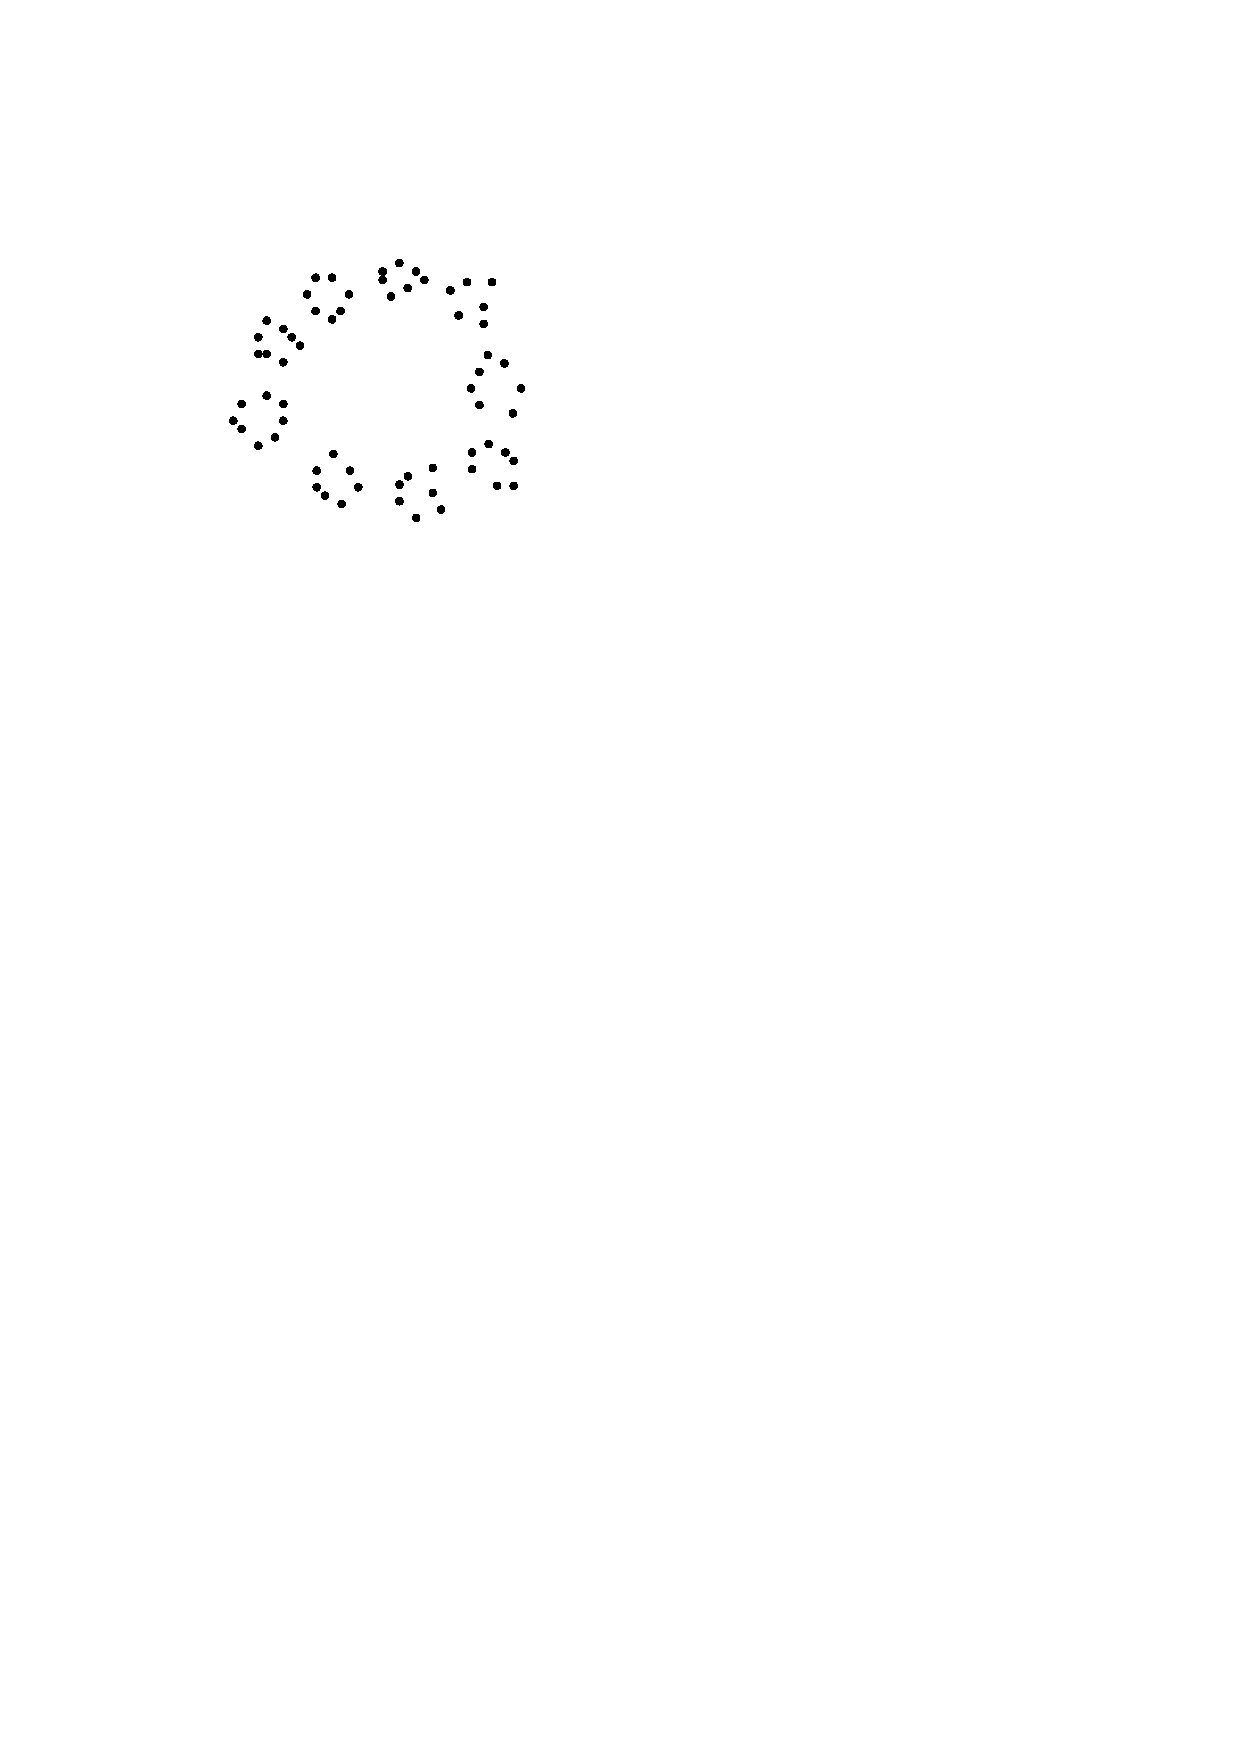
\includegraphics[width=.5\linewidth]{figures/ExampleScale}
  \captionof{figure}{%Point cloud with different topological features depending on the scale.
%It is unclear in this example what the geometric underlying object is.
This point cloud seems to be sampled on nine circles from a small scale, and on a single circle from a larger scale.}
  \label{fig:scale}
\end{minipage}
\end{figure}

Similarly, connected components, cavities
and higher-dimensional holes are topological features. In order to formalize the presence of such holes (in any dimension), 
{\em homology theory} was developed in the 19th and the beginning of the 20th century. 
It provides an algebraic encoding of such topological information. 
Basically, the homology of a space is a family of abelian groups
(one for each topological dimension), whose elements are linear combinations of the space's holes.

However, it turns out that the homology groups themselves perform poorly as topological descriptors. The main reason
is that data often comes in the form of point clouds, and the homology groups are not informative for such objects:
each point of the cloud is a generator of the 0-dimensional homology group, since 0-dimensional homology is concerned with connected 
components, and all higher-dimensional homology groups are trivial since the point cloud has no holes.
However, it may happen that the data still contains topological information, 
for instance when the point cloud is a sampling of a geometric  object such as
a circle, a sphere or a torus. 
Hence, the question that arises is that of the scale at which one should look at the data,
as illustrated in Figure~\ref{fig:scale}.

%\begin{figure}[h]\centering
%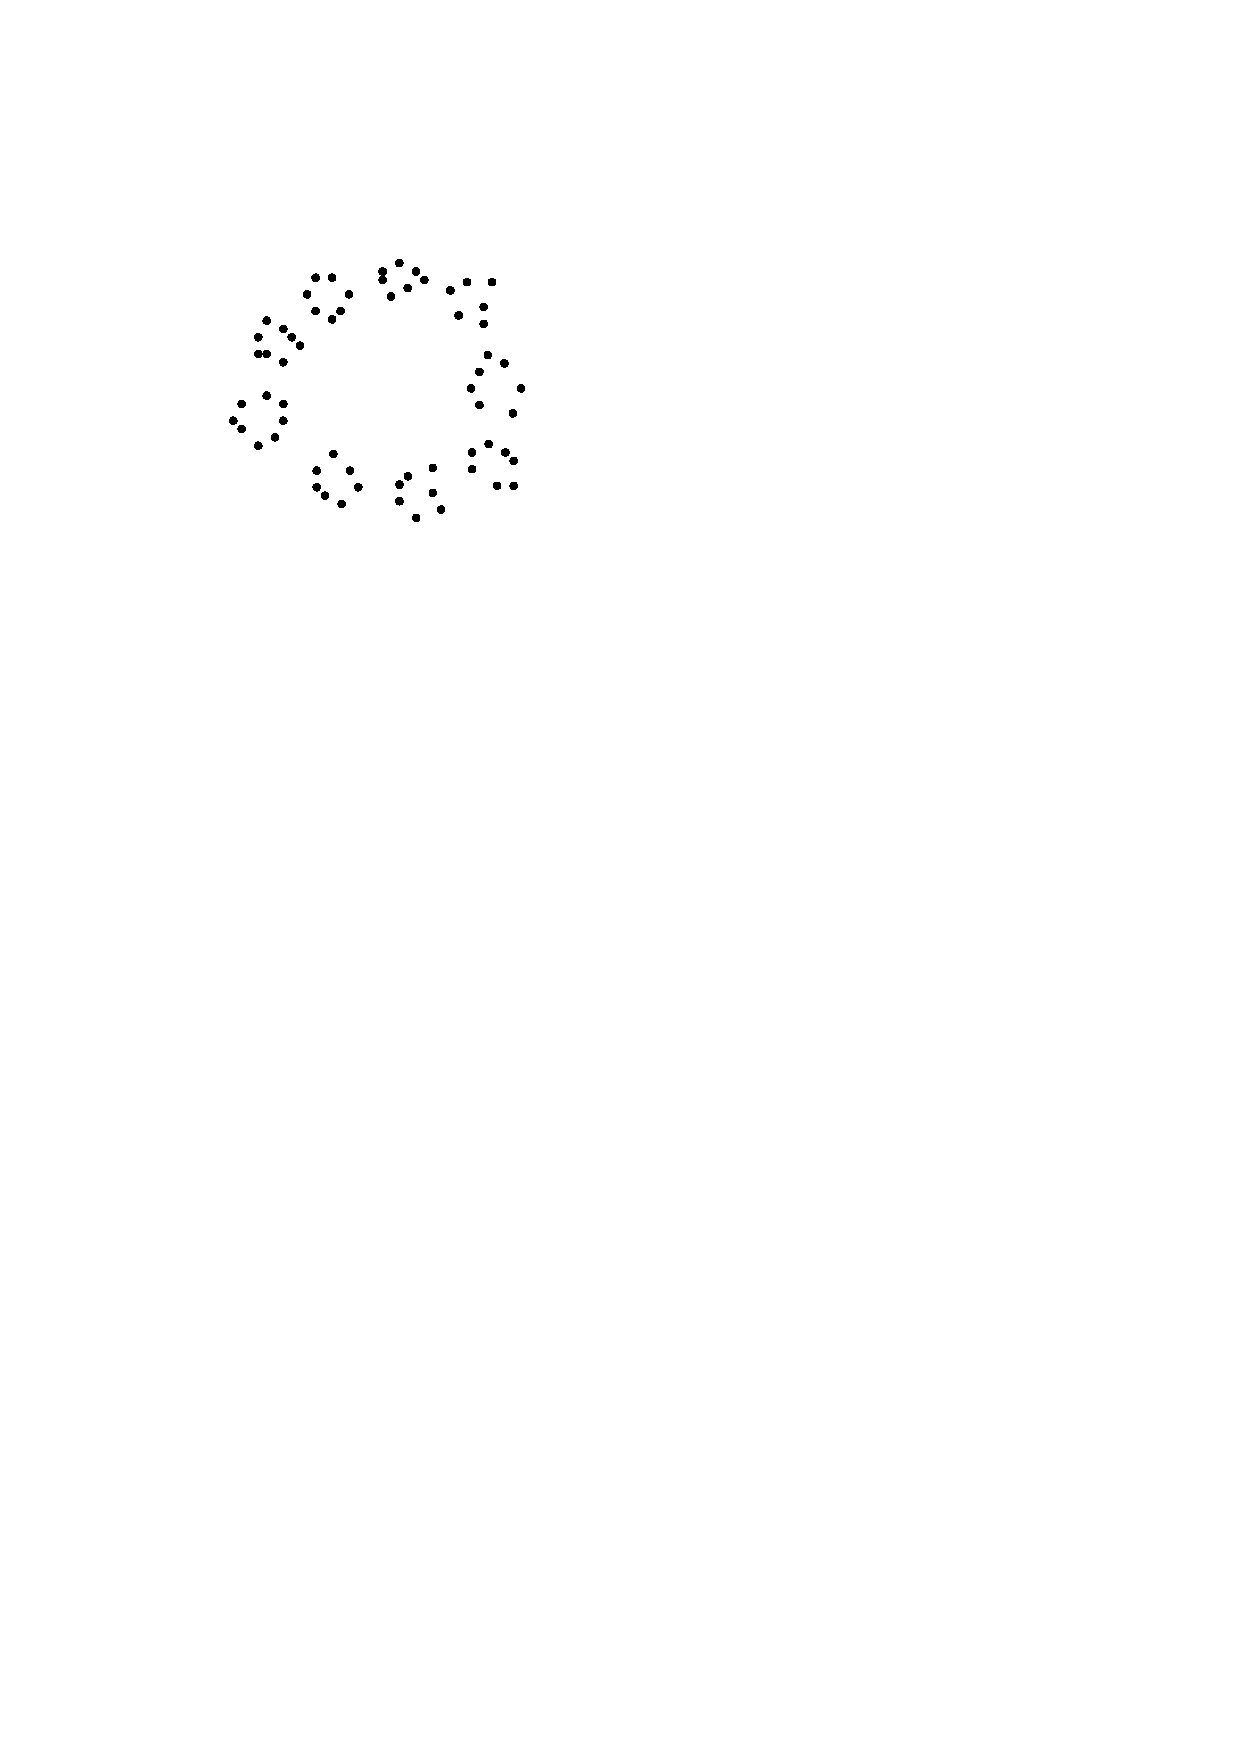
\includegraphics[height=2cm]{figures/ExampleScale}
%\caption{\label{fig:scale} It is unclear in this example what the geometric underlying object is. At small scale, it seems to be a union 
%of nine circles, whereas it would rather be a single disk at a larger scale.}
%\end{figure}

Topological data analysis provides two constructions:    
{\em persistence diagrams}, which summarize the topological information at all possible scales, and {\em Mappers},
which encode extra geometric information but at a fixed scale.



\paragraph*{Persistence diagrams.} 
Since several different scales may contain relevant topological information, the idea of persistent homology
is to encode the homology of the point cloud at all possible scales. Consider the dataset of Figure~\ref{fig:dataset},
containing images with 128 $\times$ 128 pixels, seen as 16,384-dimensional vectors, where each coordinate is the grey scale value of a pixel.
Since the camera circled around the object, 
%these images represent the same object taken from different angles, 
it follows that, from a small scale, the data looks 
composed of small clusters, each of which characterizing a specific angle, whereas from a larger scale, 
the data seems to be sampled on a circle (embedded in $\R^{16,384}$).

\begin{figure}[h]\centering
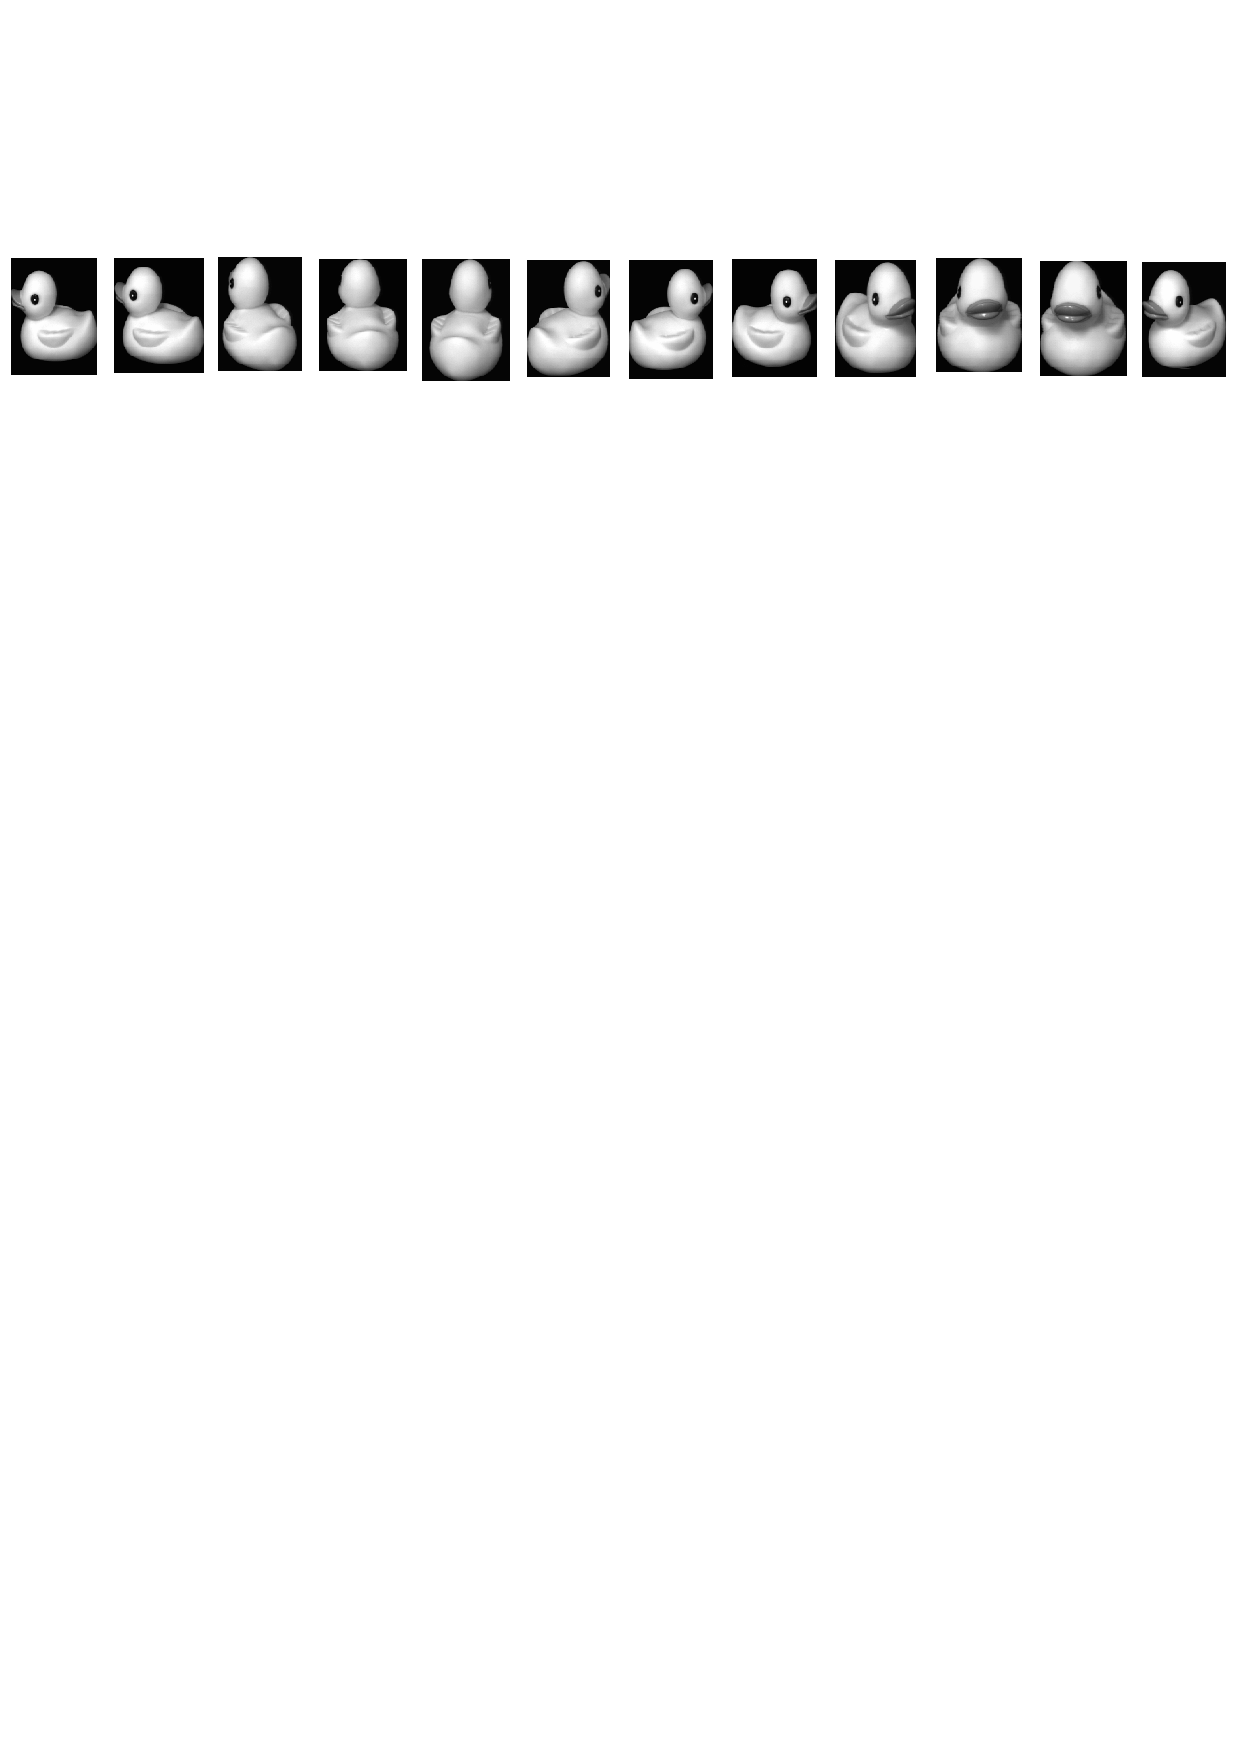
\includegraphics[width=\textwidth]{figures/ExampleDataset}
\caption{\label{fig:dataset} A dataset of images.}
\end{figure}

To summarize this information, the idea is to grow balls centered on each point of the dataset. 
Let us look at three different radius values: a small one $\alpha$, a slightly larger intermediate one $\beta$, and
a very large one $\gamma$ for these balls, as displayed in Figure~\ref{fig:ExamplePersistence}.

\begin{figure}[h]\centering
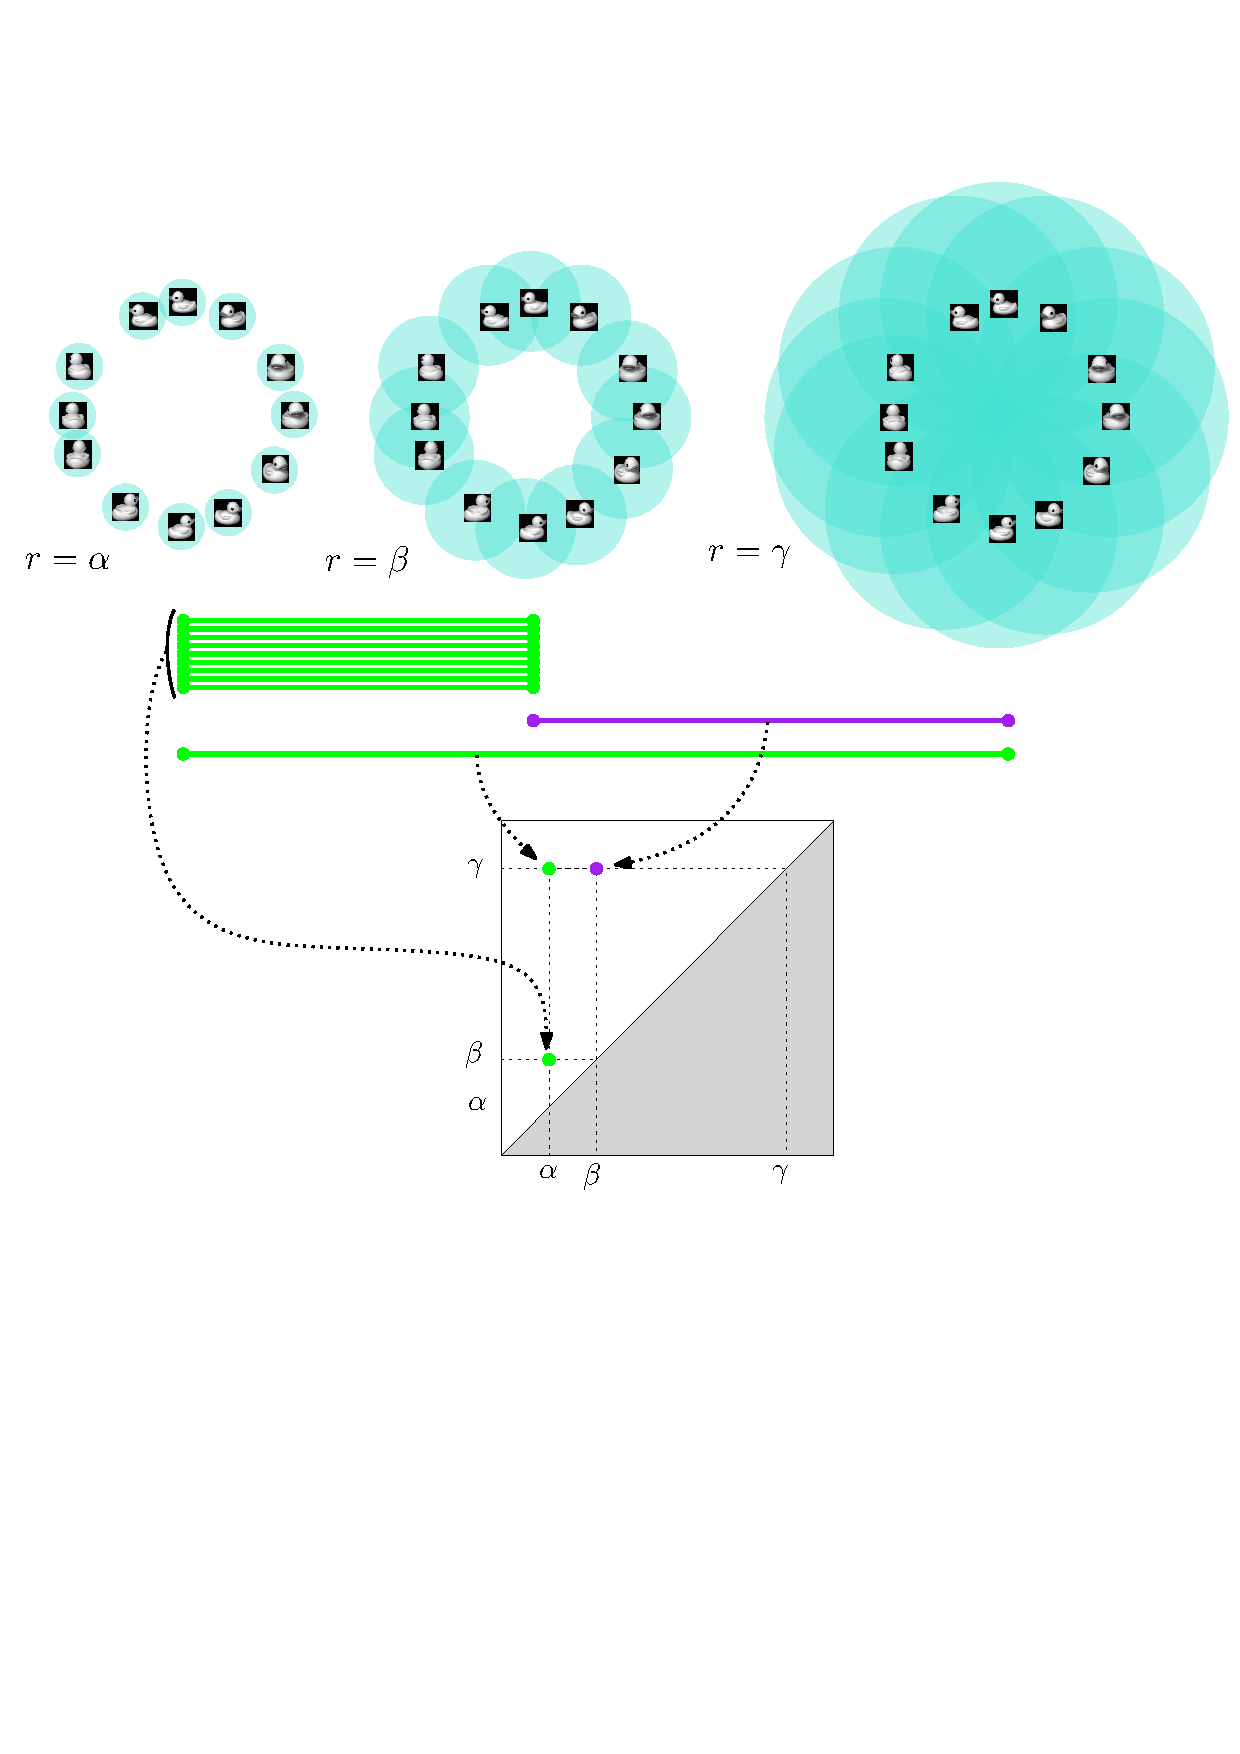
\includegraphics[width=0.8\textwidth]{figures/ExamplePersistence}
\caption[Persistence diagrams induced by growing balls]{\label{fig:ExamplePersistence} Three different unions of balls centered on images seen as vectors in high-dimensional Euclidean space.
The appearance and disappearance of topological features like connected components or holes is recorded and stored in the so-called {\em persistence diagram},
in which green points represent 0-dimensional features and purple points represent 1-dimensional features.}
\end{figure}	

When the radius of the balls is $\alpha$,
the union of balls is a just a union of ten connected components with trivial homology in dimension 1 and above.
However, when the radius is $\beta$, the union of balls has the homology of a circle, whose 1-dimensional hole
gets filled in when the radius increases to $\gamma$. Hence, we say that the connected components were born at value $\alpha$,
and nine of them died, or got merged in the tenth one, at radius $\beta$. Similarly, the 1-dimensional circle was born, or appeared, at value $\beta$ and
died, or got filled in, at value $\gamma$. Finally, the tenth connected component appeared at radius $\alpha$ and remained all the way until radius $\gamma$.
This is summarized in the {\em persistence diagram}, which is a multiset
\footnote{A multiset is a generalization of a set, in which points can have multiplicities.}
%set where one can find the same element multiple times.} 
of points, each of which 
represents a topological feature and has the birth and death radii as coordinates. 
The distance to the diagonal is a useful interpretable quantity in persistence diagrams. Indeed, if a point is far from the diagonal, then 
its ordinate, or death radius, is much larger than its abscissae, or birth radius. This means that the corresponding topological feature was
present in the union of balls for a large interval of radii, suggesting that the feature is likely to be present in the underlying object, and thus significant.
On the contrary, points close to the diagonal represent features that disappeared quickly after their appearance. These fleeting features are 
likely to be nonsignificant features or noise artifacts. Consider for instance the nine connected components in the union of balls of 
radius $\alpha$ in Figure~\ref{fig:ExamplePersistence}, which disappeared at radius $\beta$ slightly larger than $\alpha$.
Note that we explained the construction using only three unions of balls, but it is of course possible to compute
a persistence diagram when the radius increases continuously from $0$ to $+\infty$. 
In that case, 
%the tenth connected component would have coordinates $0$ and $+\infty$,
the 1-dimensional hole has an abscissa located between $\alpha$ and $\beta$ (since it is not yet present at radius $\alpha$
and already present at radius $\beta$), and an ordinate located between $\beta$ and $\gamma$ (since it is already gone at radius $\gamma$).
Similarly, all connected components have an abscissa equal to $0$. Nine of them\footnote{Actually, each point is a connected component at radius $0$.} 
have an ordinate located  between $\alpha$ and $\beta$
and the ordinate of the tenth one is $+\infty$ since it is always present, whatever the radius of the balls.

Persistence diagrams can actually be defined much more generally---even though
%we presented an example with growing balls, persistence diagrams can be defined and built over much larger classes of spaces
 the interpretation with scales may no longer be true.
All that is needed is a family of spaces which is nested with respect to the inclusion, called a {\em filtration}. 
This is a family $\{X_\alpha\}_{\alpha\in A}$, where 
$A$ is a totally ordered index set, such that $\alpha\leq\beta\Rightarrow X_\alpha\subseteq X_\beta$.
Then, the construction of persistence diagrams remains the same, i.e. keeping track of the appearance and disappearance of topological features
as we go through all indices in ascending order.
In the previous example, the filtration had three elements,
the three different unions of balls, each union being indexed by the radius of its balls.
It is clear in this case that these three spaces are nested since a ball
is always included in the ball with same center and larger radius.

A common way to build a filtration is to use the {\em sublevel sets} of a continuous scalar-valued function $f$, which are sets of the form
$f^{-1}((-\infty,\alpha])$. Indeed, it is clear that $f^{-1}((-\infty,\alpha])\subseteq f^{-1}((-\infty,\beta])$ for any $\alpha\leq\beta\in\R$. 
%This is the case for the filtration induced by taking unions of balls. Indeed,   
%with radius $r$ centered on points of $P$: $\cup_{p\in P}B(p,r)$, 
For instance, the union of balls with radius $r$ centered on the points of a point cloud $P$
is equal to the sublevel set of the distance function to  $P$: $d_P^{-1}((-\infty,r])$, where $d_P(x)=\min_{p\in P}d(x,p)$.
Hence, as soon as there is a continuous scalar-valued function at hand, a persistence diagram can be computed, which explains
why the persistence diagram is a versatile descriptor. %that can be used not only for datasets, but also for data points. 
Consider for instance the blurry image of a zero in the down right corner of Figure~\ref{fig:blurryzero}, where
the grey value function is used to compute the persistence diagram. Again, there are two points standing out
in the persistence diagram, one representing the connected component of the zero, and the other representing 
the 1-dimensional hole induced by the zero. All other points are noise. 

%\begin{figure}[h]\centering
%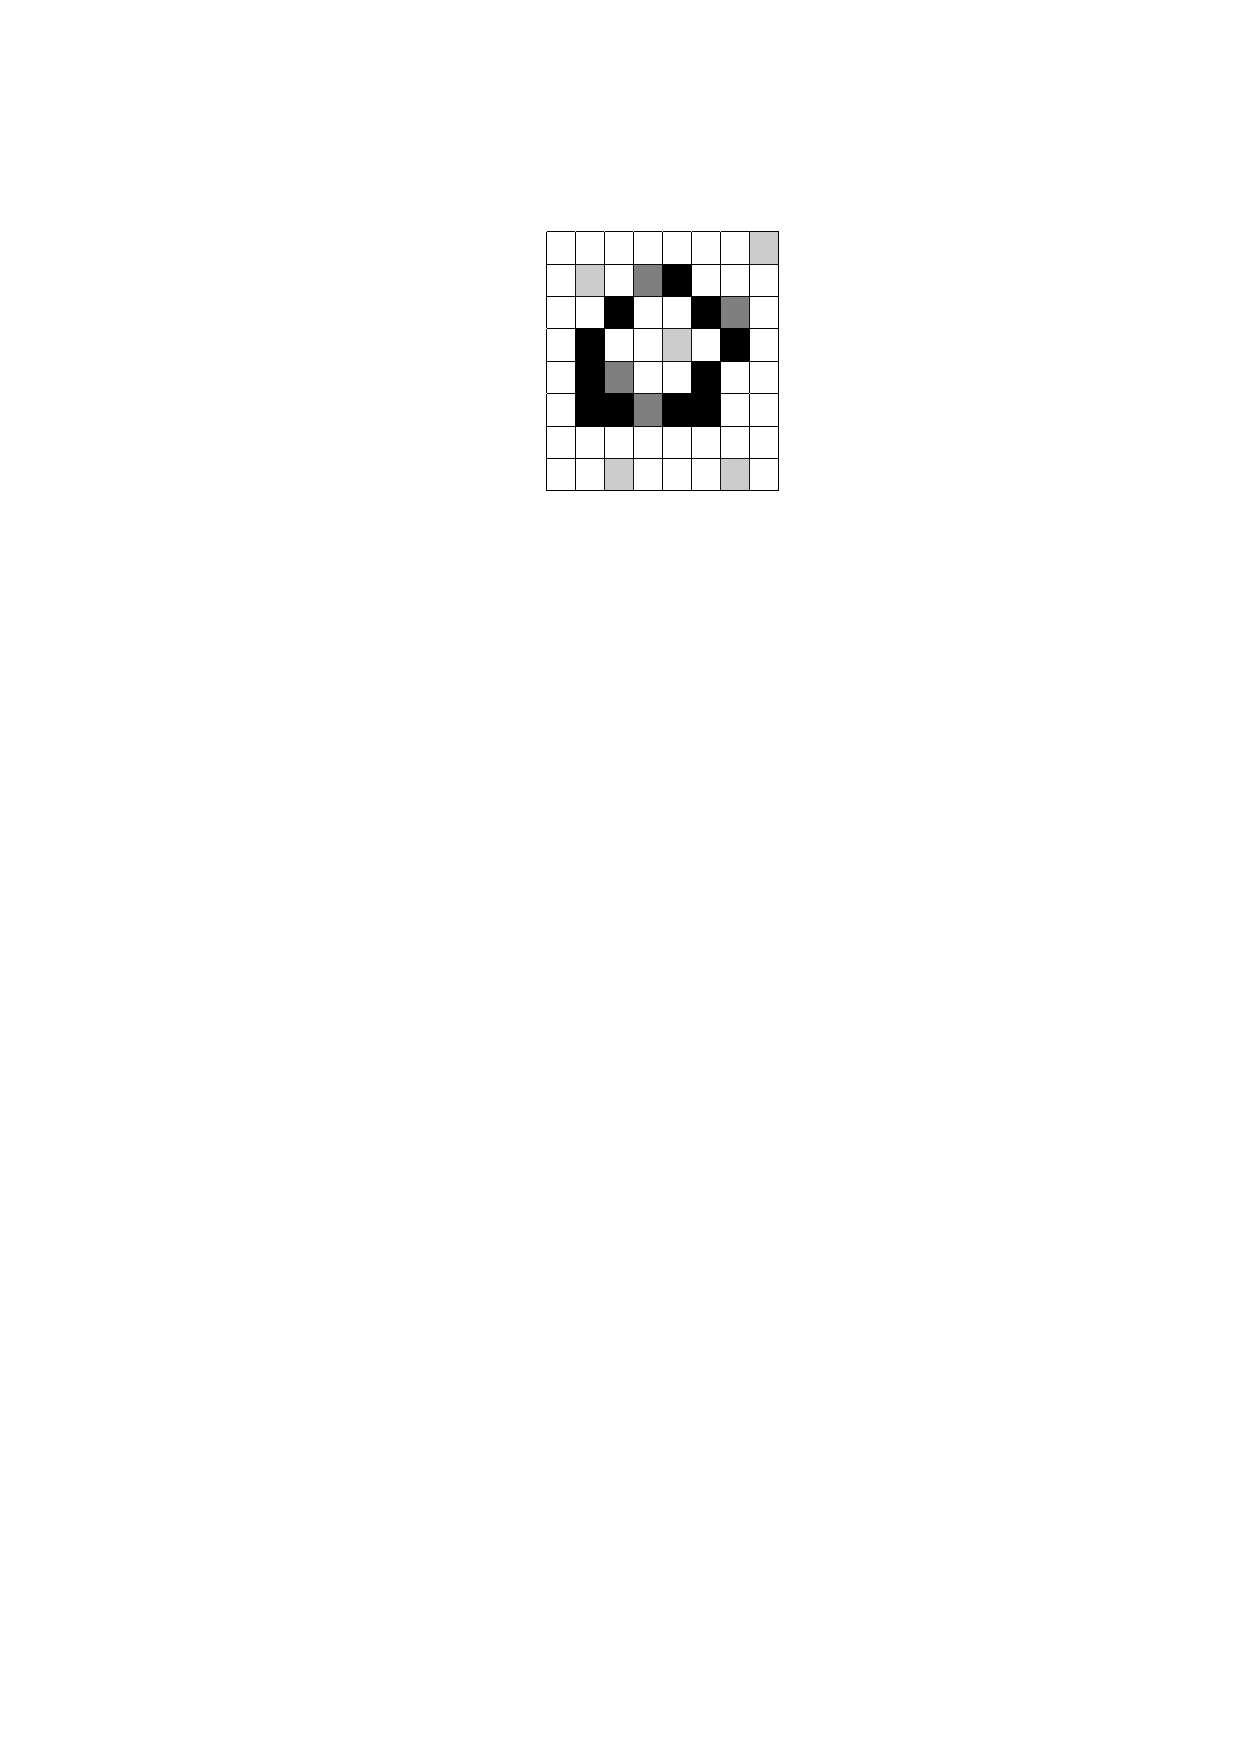
\includegraphics[width=5cm]{figures/ExampleImage}
%\caption{\label{fig:blurryzero}}
%\end{figure} 

\begin{figure}[h]\centering
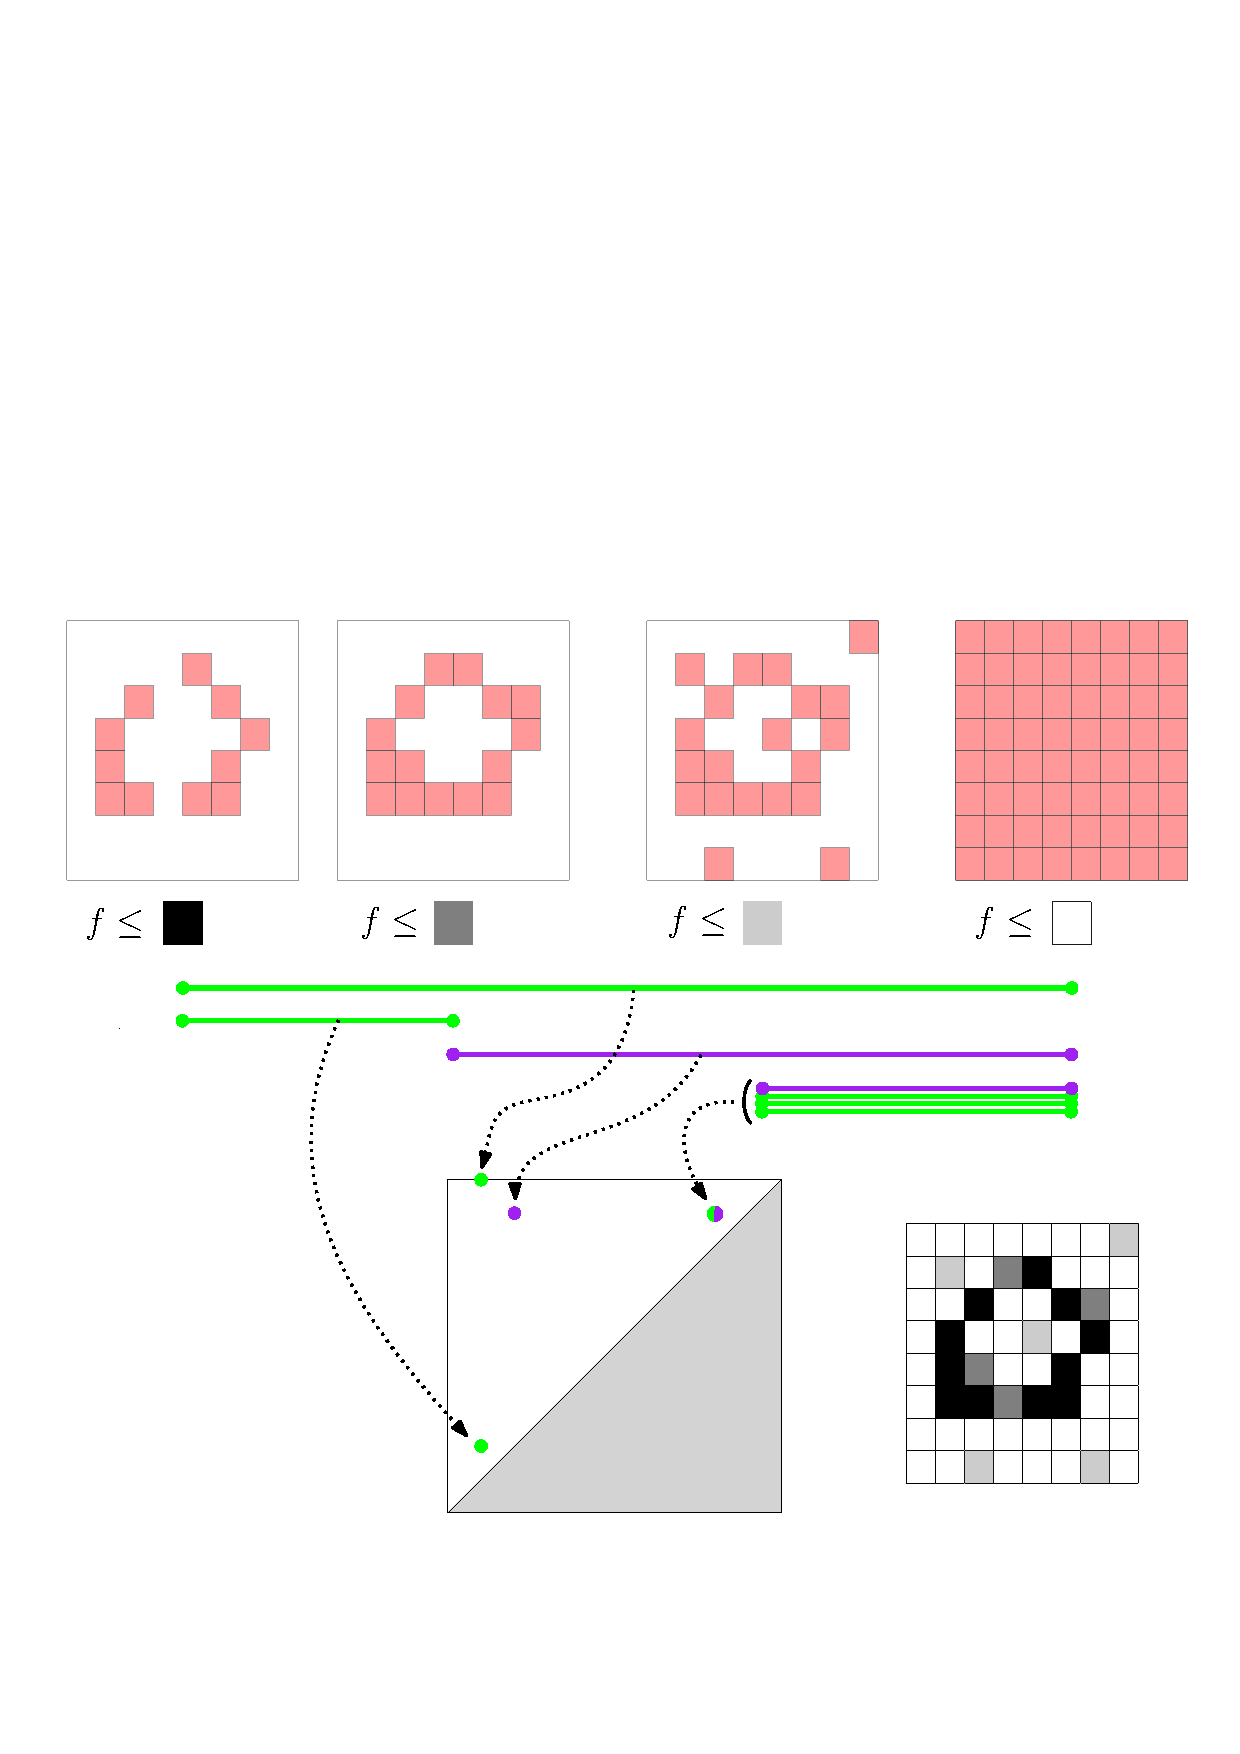
\includegraphics[width=0.8\textwidth]{figures/ExamplePersistence2}
\caption[Persistence diagram of image]{\label{fig:blurryzero} Another example of a persistence diagram construction with the sublevel sets of the 
grey value function defined on a blurry image of a zero.}
\end{figure}	

One of the reasons why persistence diagrams are useful descriptors is that, in addition to be invariant to continuous deformations (that do not involve tearing or gluing), 
they are {\em stable}~\cite{Chazal09a,Cohen07}. Indeed, if persistence diagrams
are computed with sublevel sets of similar functions, 
then the distance between them  is upper bounded by the difference between the functions in the sup norm:
$$\distb(\dg(f),\dg(g))\leq \|f-g\|_\infty,$$ where $\distb$ stands for the bottleneck distance between persistence diagrams,
which is the cost of the best partial matching that one can find between the points of the persistence diagrams.
This means that, for instance, if the positions of the images in Figure~\ref{fig:ExamplePersistence} are slightly perturbed, 
or if the blurry image of a zero in Figure~\ref{fig:blurryzero} is slightly changed, then the 
resulting persistence diagrams will end up very close to the original ones in the bottleneck distance.
%corresponding  distance function to the perturbed point cloud,
%or the grey value function of the smoothed image
%is going to be very similar to the original one and the  
%are compared with suitable metrics, like the bottleneck or Wasserstein distances, 


Persistence diagrams have proven
useful %and helped improve data analysis 
in many data analysis applications, ranging from 3D shape analysis~\cite{Carriere15a, Chazal09c} 
%to medical diagnosis~\cite{Lum13,Nicolau11,Rucco15} 
to glass material transition~\cite{Gameiro16, Hiraoka16} to genomics~\cite{Camara16,Chan13}, to name a few. 
  
   

%\begin{figure}
%\includegraphics[width=15cm]{figures/ExamplePersistencealt}
%\includegraphics[width=5cm]{figures/ExamplePersistencealt2}
%\includegraphics[width=5cm]{figures/ExamplePersistencealt3}
%\end{figure}

 


\paragraph*{Mapper.} As explained above, persistence diagrams summarize the topological information in data.
However, they lose a lot of geometric information in the process: it is easy to build different spaces with the same persistence diagrams.
The {\em Mapper}\footnote{In this thesis, we call {\em Mapper} the
mathematical object, not the algorithm used to build it.}, 
which was introduced in~\cite{Singh07}, is a direct approximation of the underlying object. It encompasses not only the topological features,
but also additional information, on how the features are positioned with respect to each other for instance.
As with persistence diagrams, a continuous scalar-valued function, sometimes called {\em filter}, is needed, as well as a cover of 
its image with open overlapping intervals.
The idea is to compute the preimages by $f$ of all intervals in the cover, to apply clustering on these preimages in order to refine them into connected components,
and finally to link the connected components if they contain data points in common.  

\begin{figure}[h]\centering
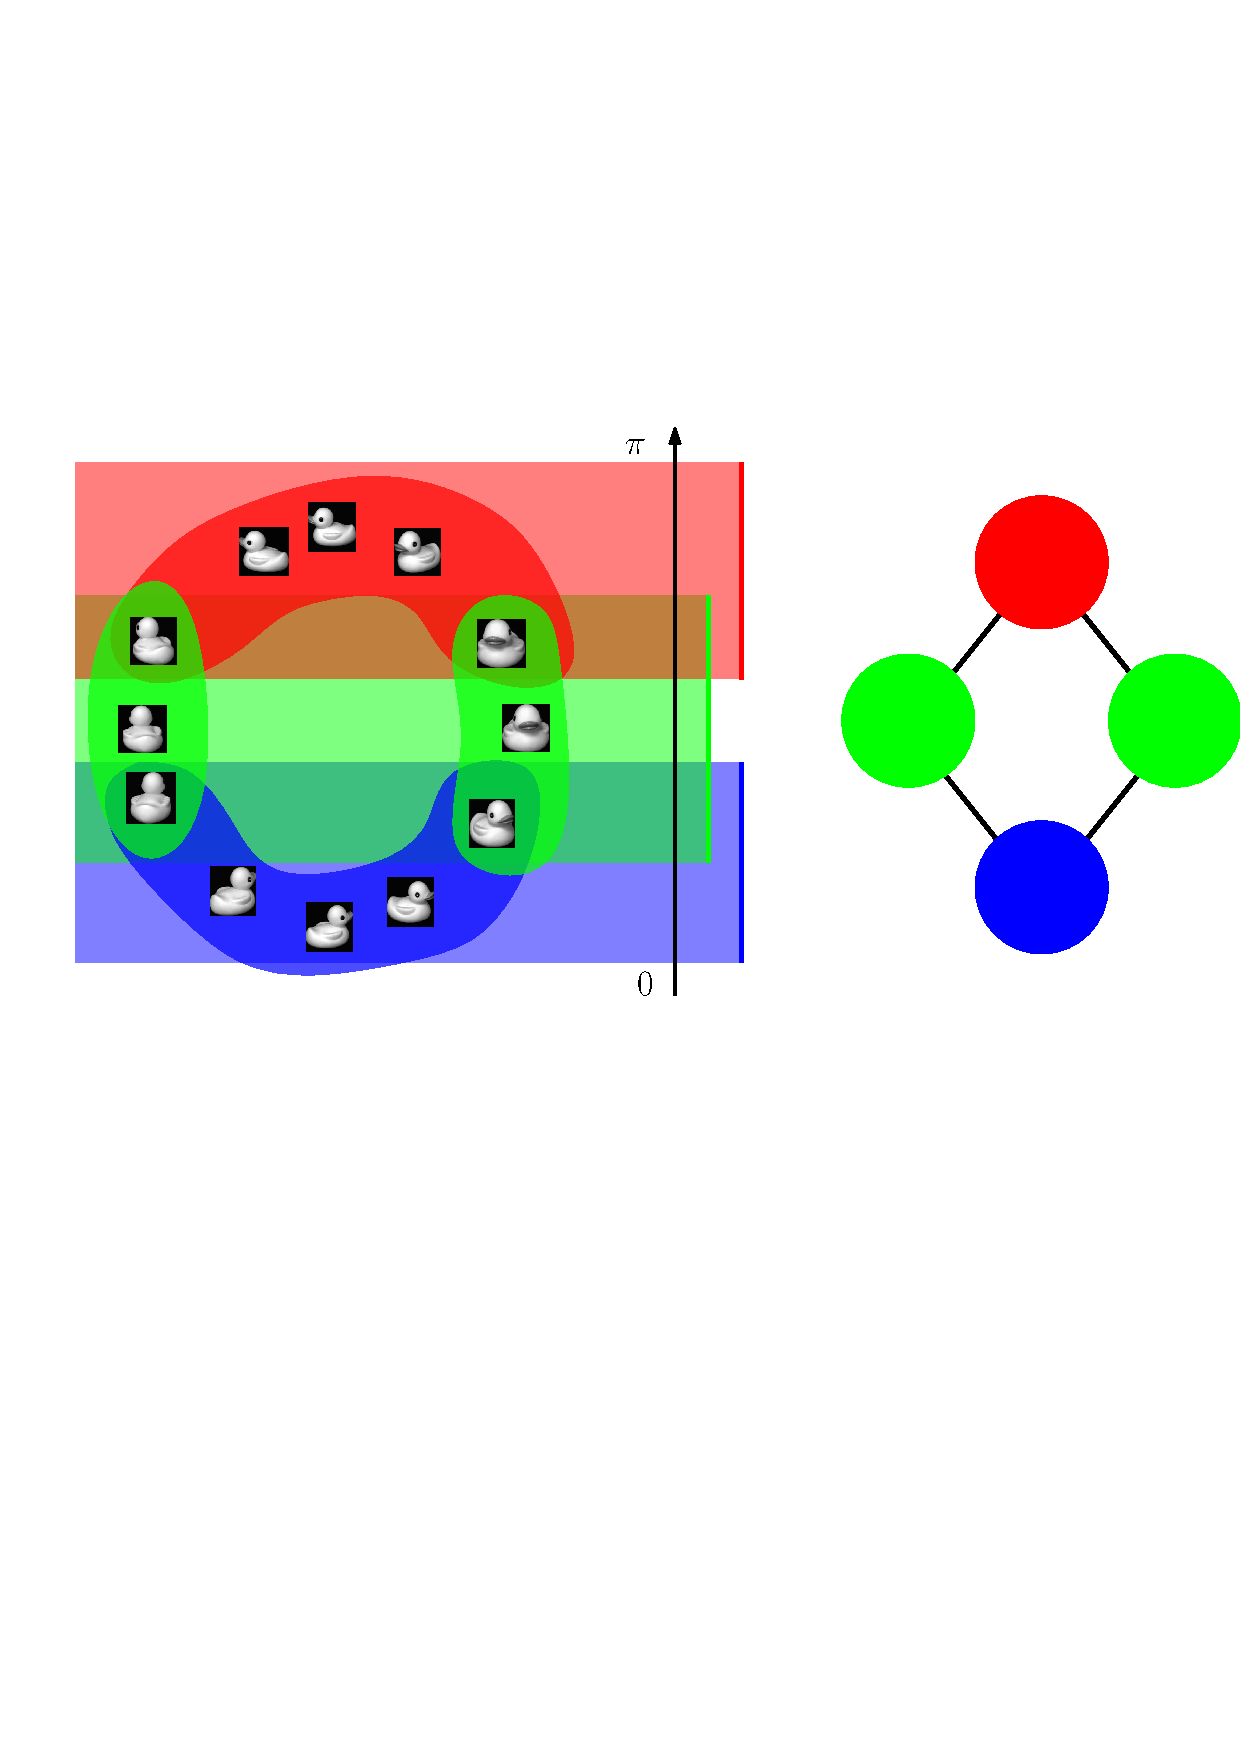
\includegraphics[width=.75\textwidth]{figures/ExampleMapper}
\caption[Mapper on images]{\label{fig:mapper}Example of Mapper computed on the point cloud of images with the angle function and a cover of three intervals.}
\end{figure}	

We provide an example in Figure~\ref{fig:mapper}, where we consider again the point cloud of images. The continuous scalar-valued function is 
the absolute value of the angle at which the picture was taken, and its image $[0,\pi]$ is covered by three intervals (blue, green and red). 
In the preimage of the red and blue intervals there is just one connected component, whereas there are two in the preimage of the green interval.
We obtain the Mapper by putting edges between the connected components according to whether they share data points or not; for instance, 
the green and blue or green and red connected components are linked whereas the red and blue are not. The Mapper has the homology of the circle, and is a 
direct approximation of the underlying support of the point cloud. 

Note that the lengths of the intervals in the cover directly control the scale at which the data is observed: if the intervals are very small, the Mapper
will have many disconnected nodes since the preimages of the intervals will contain at most one point. 
On the opposite, if the intervals have large lengths,
the Mapper will have only few nodes since the preimages of the intervals are going to contain many points.  
%The best interval length, the one for which the Mapper is close to the underlying object, is somewhere in the middle. 

%Note that the Mapper can be defined more generally for functions taking values in $\R^D$ instead of $\R$. Then the output may be a simplicial complex
%of dimension larger than one instead of a graph. 

%\subsection{Machine Learning}
%Once data is synthetized in a suitable descriptor, it can be processed efficiently with Machine Learning.
%{\em Machine Learning} is a field of data analysis which aims at predicting new data from already collected data. 
%The core idea of Machine Learning is to derive structure and information from already collected data, and then use this information
%so as to be able 

In practice, the Mapper has two major applications. The first one is data visualization and clustering.
Indeed, when the cover $\I$ is minimal, the Mapper provides a visualization of the data in the form of a graph whose topology reflects
that of the data. As such, it brings additional information to the usual clustering algorithms 
about the internal structure of the clusters, 
by identifying {\em flares} and {\em loops} that outline potentially remarkable topological information
in the various clusters. See e.g.~\cite{Yao09, Lum13, Sarikonda14, Hinks15} for examples of applications. 
The second application of Mapper deals with feature selection. Indeed,
each feature of the data can be evaluated on its ability to discriminate  
the topological features mentioned above (flares, loops) from the rest of the data, 
using for instance Kolmogorov-Smirnov tests.
See e.g.~\cite{Lum13, Nielson15, Rucco15} for examples of applications.   
%Unsupervised methods generally depend on parameters that 
%need to be chosen by the user. For instance, the number of selected dimensions for dimension reduction 
%methods or the number of clusters for clustering methods have to be chosen. 
%Contrarily to supervised problems, it is tricky to evaluate the output of unsupervised methods and thus to select parameters. 


\subsection{Main bottlenecks}

Even though Mapper and persistence diagrams enjoy many desireable properties, several limitations
%slightly jeopardize
hinder their effective use in practice, in particular the {\em difficulty to set the parameters for Mapper}
%{\em lack of distance and stability results} for Mapper
and the {\em non linearity} of the space of persistence diagrams. 

\paragraph*{Distances and stability for Mappers and Reeb graphs.}
%
One problem with the Mapper is that, contrary to the persistence diagrams, it has a parameter, which is the cover,
and it is unclear how this cover should be tuned beforehand.
Because of this, %arbitrary fixed cover, or scale,
the Mapper seems to be a very {\em unstable} construction:
%Indeed, a Mapper needs an arbitrary choice of cover, or scale, to be computed. Hence, 
it may happen that Mappers computed on nearby point clouds, 
as in Figure~\ref{fig:instabMapper}, or with similar covers, as in Figure~\ref{fig:instab},
end up being very different.

\begin{figure}[h]\centering
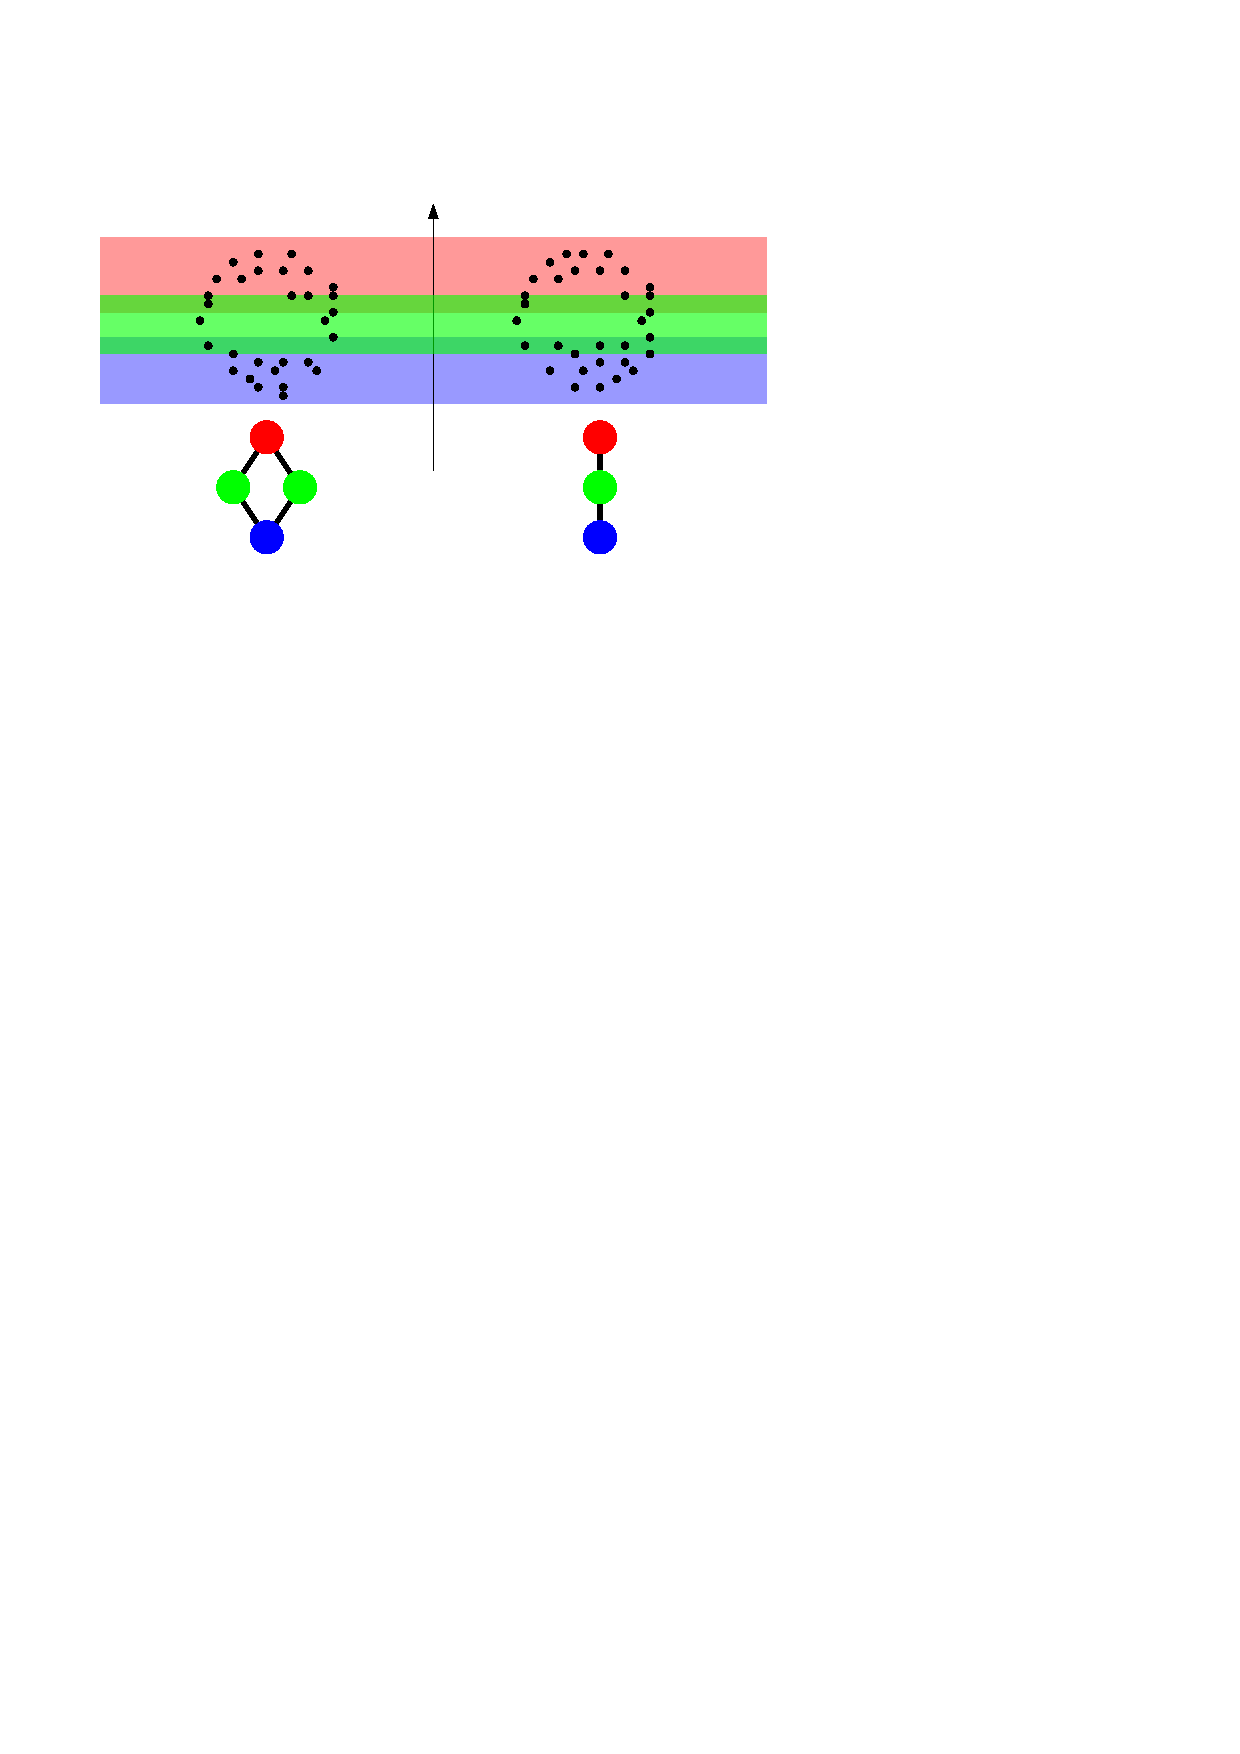
\includegraphics[width=10cm]{figures/ExampleInstabilityMapper}
\caption[Instability of Mapper computed on nearby spaces]{\label{fig:instabMapper} Mappers of two similar samplings of the circle, computed with the height function
and a cover with three intervals.}
\end{figure}

%This situation is highly problematic with Mapper since, as for many topological methods, it is not robust to outliers. 
This major drawback of Mapper is an important obstacle to its use  
in exploratory data analysis with non trivial datasets. %We give another illustration of this phenomenon  on a dataset that we study further in Chapter~\ref{chap:MapperStatistic}. 
The only answer proposed to 
this drawback in the literature consists in selecting parameters in a range of values for which 
the Mapper seems to be stable---see for instance~\cite{Nielson15}. 
%We believe that such an approach is not satisfactory because it does not provide statistical guarantees on the inferred Mapper.

\begin{figure}
\begin{tabular}{cc}
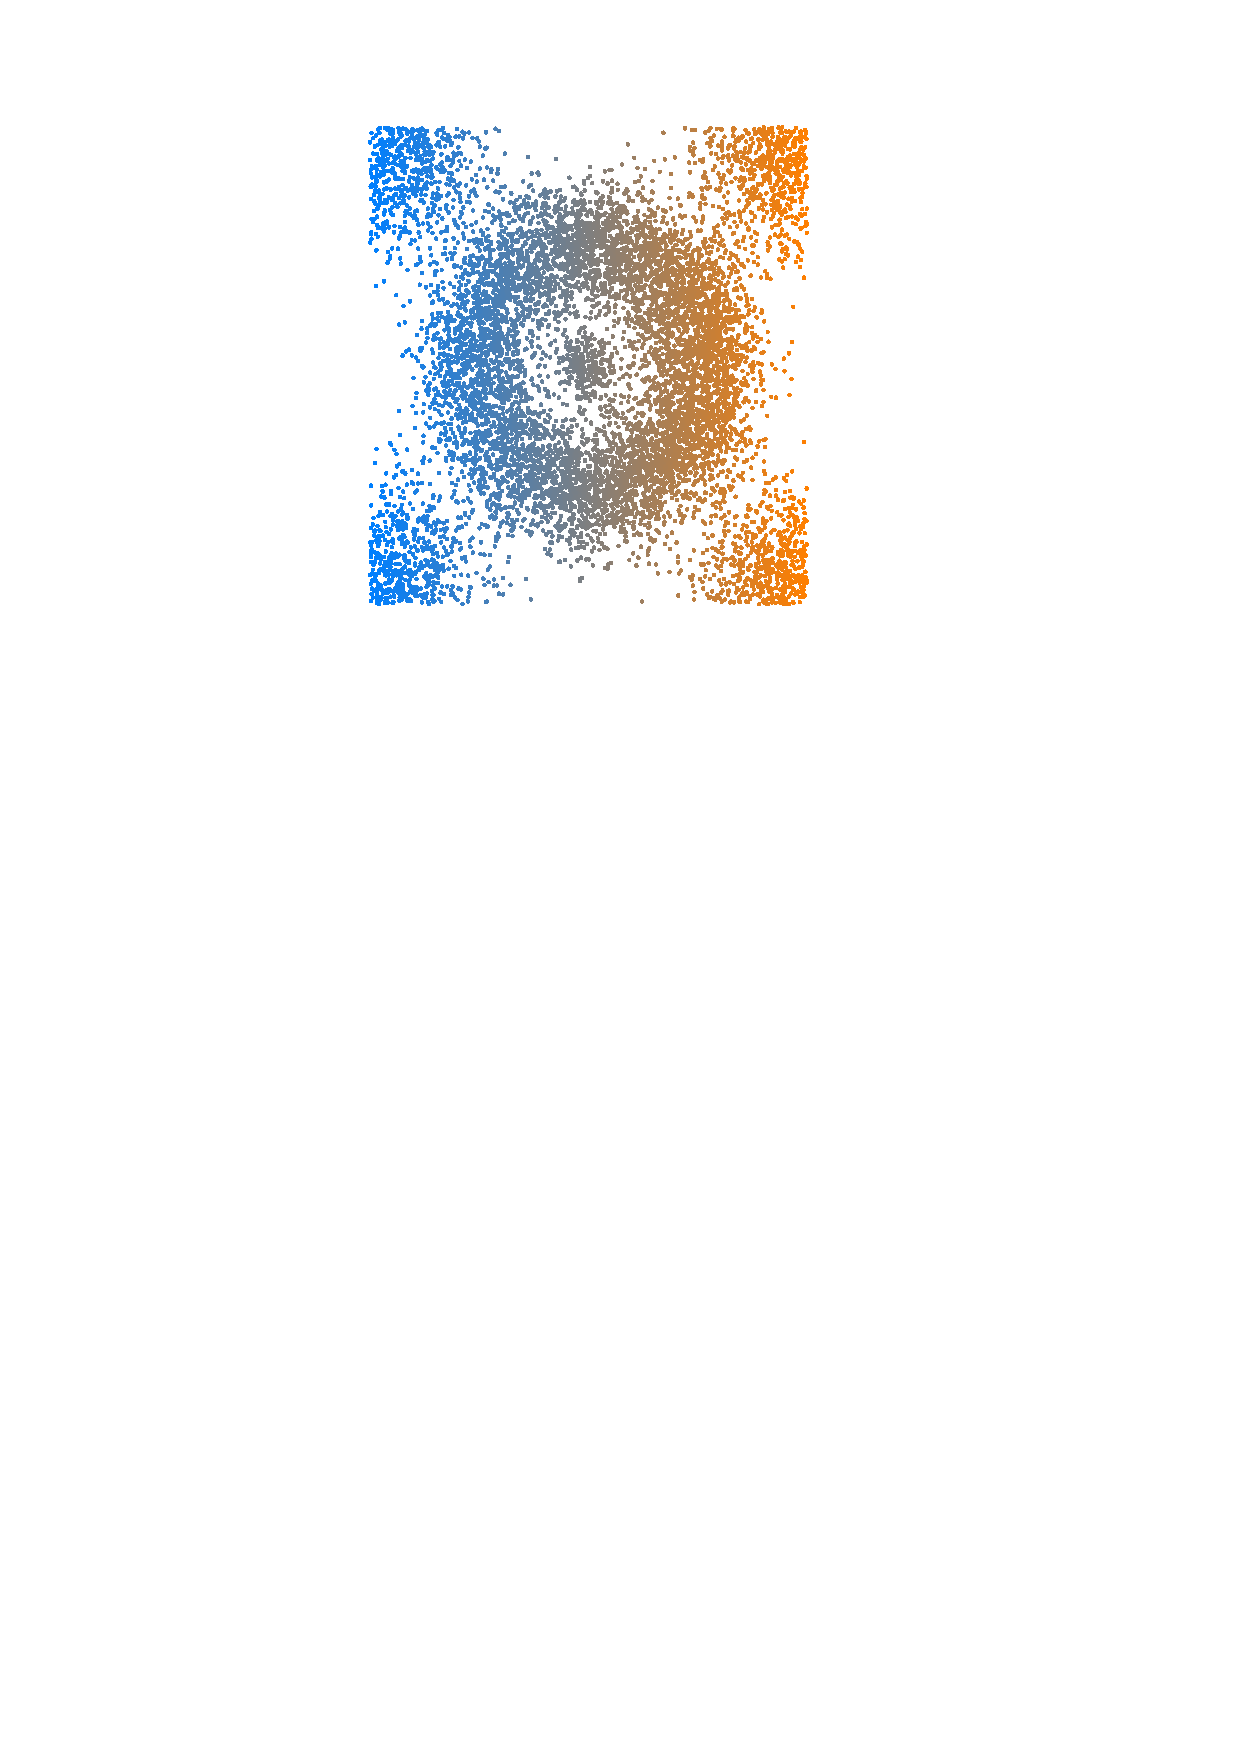
\includegraphics[width=6cm]{figures/crater_instab} & 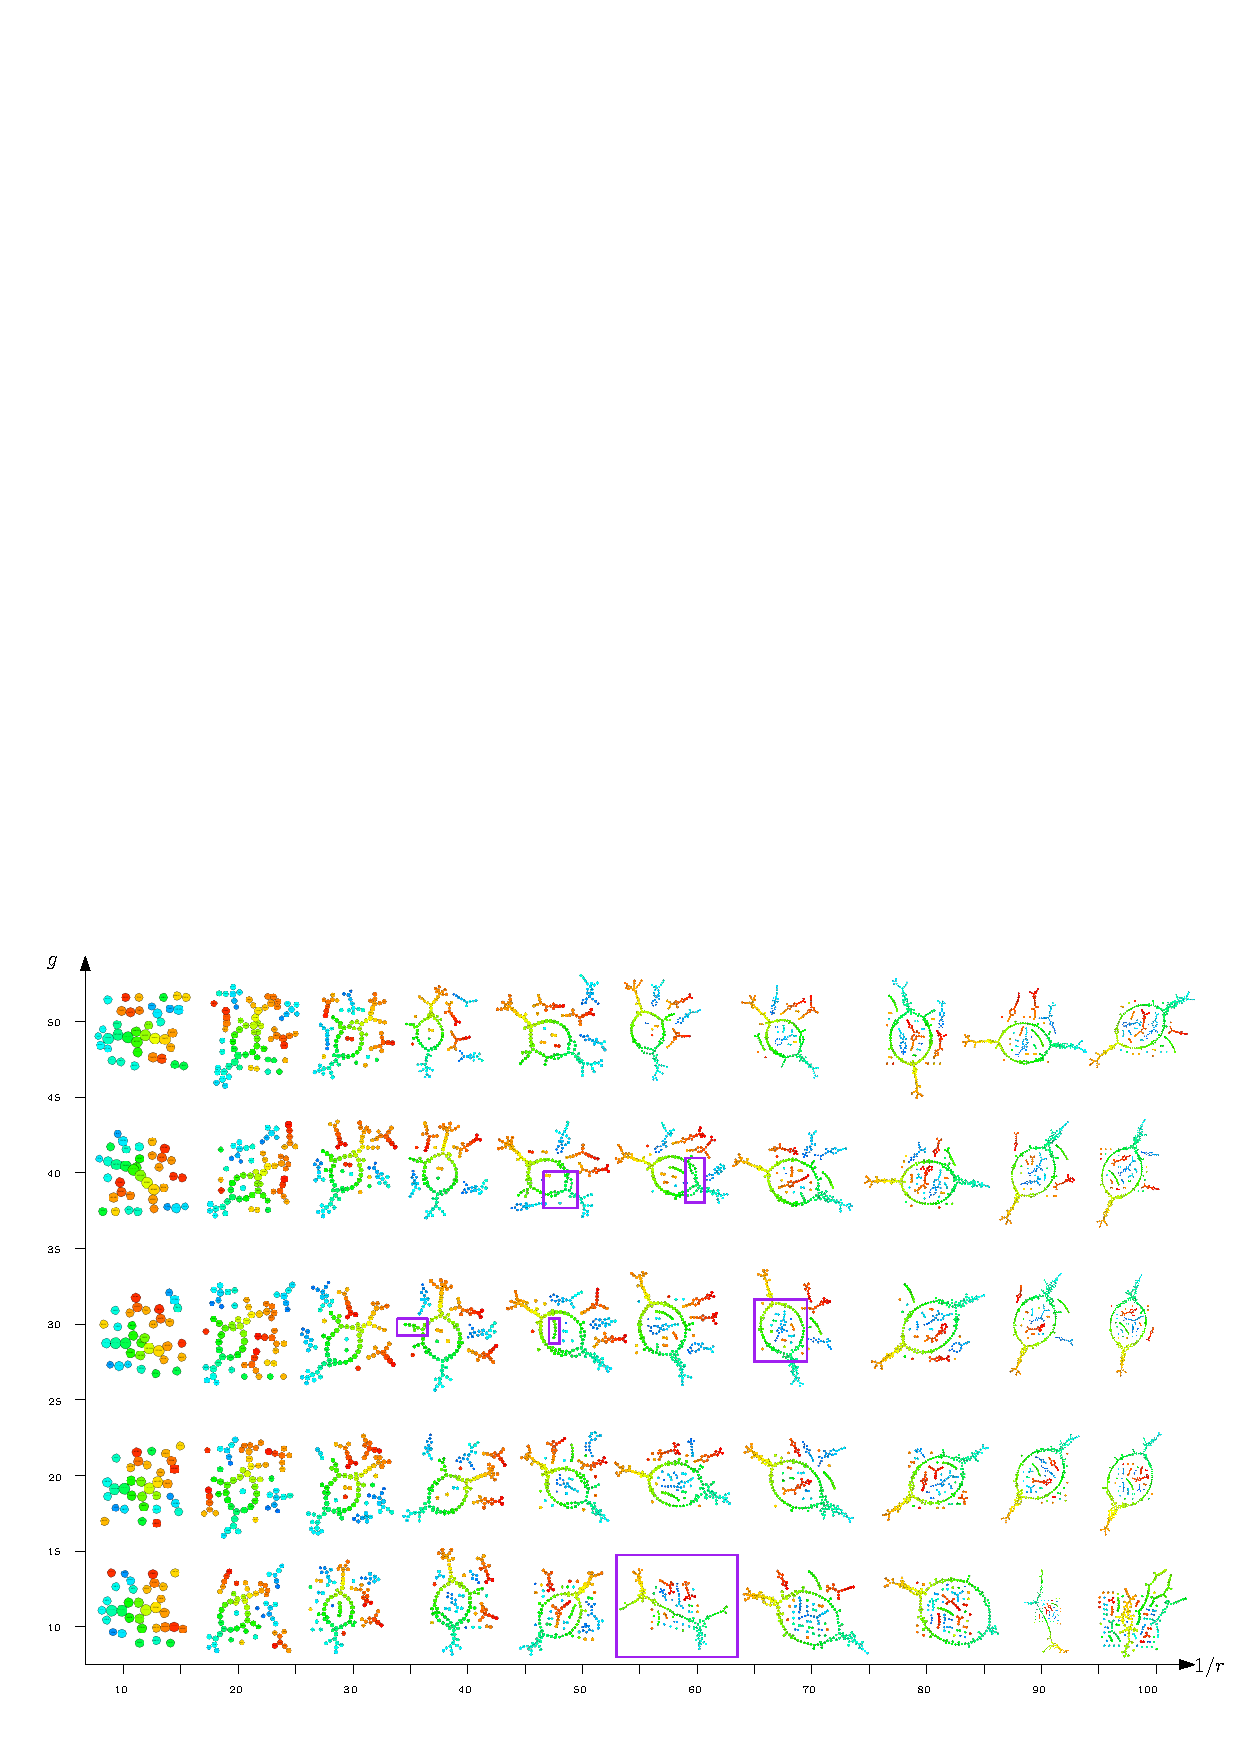
\includegraphics[width=10cm]{figures/instab}
\end{tabular}
\caption[Instability of Mapper computed with close covers]{\label{fig:instab}
A collection of Mappers of the crater dataset computed with various covers ($r$ is the length of the intervals and $g$ is their overlap percentage)
and the horizontal coordinate.
Left: crater dataset colored with function values, from blue to orange. Right: Mappers computed with various parameters. 
%One can see that for some Mappers,
The purple squares indicate topological features that suddenly appear and disappear in the Mappers. 
%These are discretization artifacts, that we overcome in this Chapter by appropriately tuning the parameters.
}
\end{figure}


Hence, deriving a stability theorem for Mappers would require to compare them with a metric that depends at least on the cover. 
Unfortunately, even though theoretical metrics can be defined, see e.g.~\cite{Munch16}, a computable and interpretable metric between Mappers is still lacking in the literature. 
To tackle this problem, one can take inspiration from another class of descriptors, which are very similar to Mappers: the {\em Reeb graphs}.

\paragraph*{Reeb graphs.} Note that the Mapper construction was originally defined for point clouds, but it can straightforwardly be extended to possibly
non discrete topological spaces, for which clustering is not needed to compute the connected components of preimages.
In that case, making the lengths of cover intervals go to zero leads to a limit object called the {\em Reeb graph}.
%It can be equivalently defined as a quotient space computed by gluing together all
%points belonging to the same connected component of a level set of the filter: $f^{-1}(\alpha)$ where $\alpha\in\R$.
Hence, Mappers (computed on non discrete topological spaces) are nothing but {\em approximations}, or 
{\em pixelized versions} of Reeb graphs, as illustrated in Figure~\ref{fig:pixelization}.

\begin{figure}[h]\centering
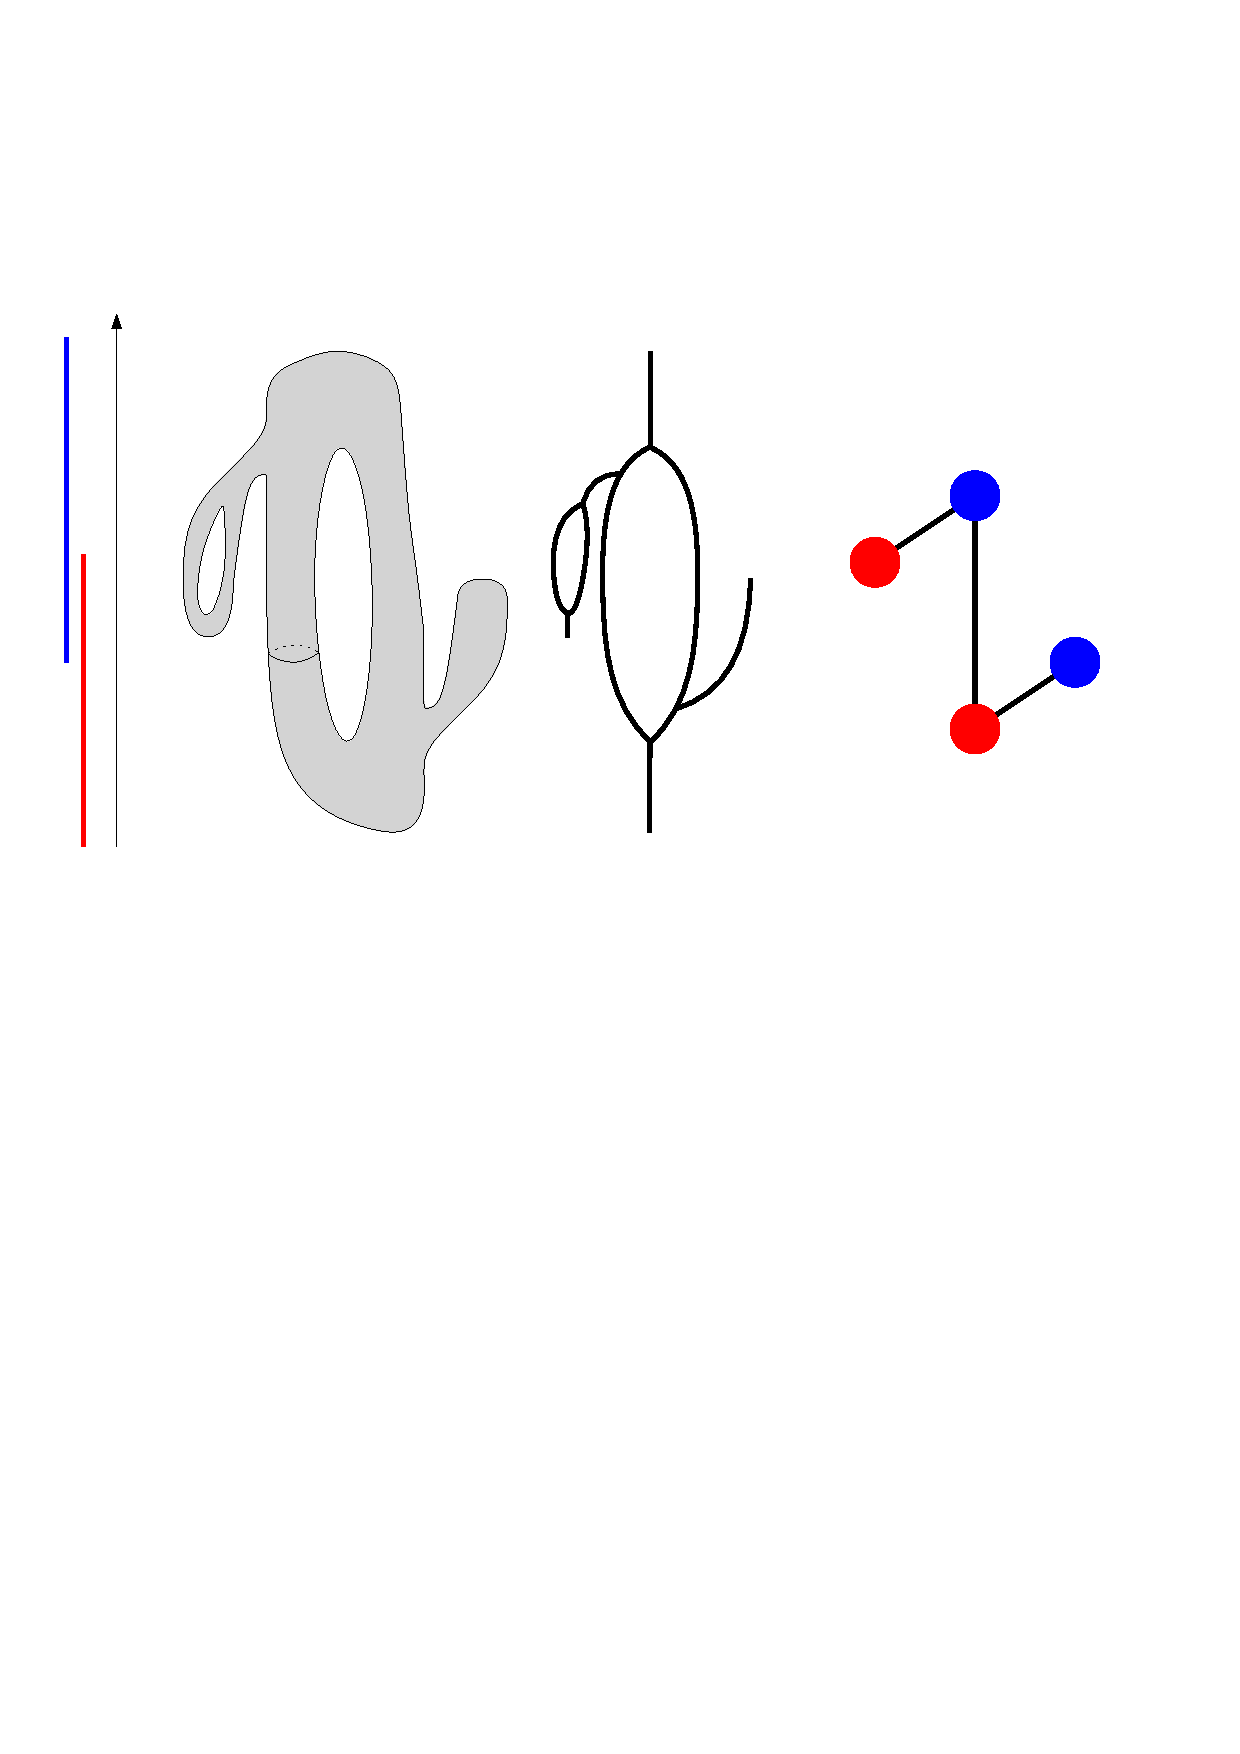
\includegraphics[width=10cm]{figures/ExamplePixelization}
\caption[Mapper as a pixelization of the Reeb graph]{\label{fig:pixelization} A surface embedded in $\R^3$ (left), its Reeb graph (middle) computed with the height function and 
its Mapper (right) computed with the height function and a cover with two intervals.}
\end{figure}
  
This observation is important since several natural metrics enjoying stability properties already exist for Reeb graphs~\cite{Bauer16,Bauer14,deSilva16}
and can be extended to Mappers. 
However, these metrics are not computable and thus cannot be used as is in practice~\cite{Agarwal15}. Hence, there is an open question about how
to define metrics for Mappers which would be both computable and stable.


  
%from the continuous
%\footnote{By continuous, we mean computable on possibly non discrete topological spaces.} counterpart of Mapper, 
%called the {\em Reeb graph}: the Reeb graph of a topological space is computed by   It can be 
%seen as a Mapper computed with open intervals whose length is infinitely small. 
%Alternatively, the Mapper can be seen as a {\em pixelized} version of the Reeb graph. 
%The problem is that of the distance used to compare Mappers. Indeed, it is unclear how to properly measure the similarity of Mappers. 
%In order to obtain a stability result similar to that of persistence diagrams,
%a suitable distance should depend on the cover used to compute the Mappers. 

\paragraph*{Non linearity of the space of  persistence diagrams.}
%
Even though persistence diagrams are stable descriptors, they cannot be plugged systematically into Machine Learning algorithms.
Indeed, a large class of these algorithms require the data to lie either in Euclidean space (such as random forests), 
or at least in a Hilbert space (such as SVM).
However, the space of persistence diagrams, equipped with the bottleneck distance, is neither Euclidean nor Hilbert.
Even Fr\'echet means are not well-defined~\cite{Turner14}. Fortunately,
the {\em kernel trick} allows us to handle this kind of data.
Assuming data points lie in some metric space $(X,d_X)$, the kernel trick only requires a positive semi-definite function,  
called a {\em kernel}. This is a function $k:X\times X\rightarrow\R$ such that, for any $a_1,\cdots,a_n\in\R$ and $x_1,\cdots,x_n\in X$:
$$\sum_{i,j}a_ia_jk(x_i,x_j)\geq 0.$$ 
Due to Moore-Aronszajn's theorem~\cite{Aronszajn50}, kernel values can be proven equal to the evaluation
of the scalar product between embeddings of data into a specific Hilbert space that depends only on $k$ and is generally unknown. 
More formally, there exists a Hilbert space $\mathcal H_k$ such that, for any $x,y\in X$: 
$$k(x,y)=\langle\Phi_k(x),\Phi_k(y)\rangle_{\mathcal H_k},$$
where the embedding $\Phi_k$ is called the {\em feature map} of $k$.
Kernel values can thus be seen as generalized scalar products between data points, and can be directly plugged into Machine Learning algorithms. 
Hence, in our case, the question becomes that of finding kernels for persistence diagrams.

A common way to define kernels for points lying in a metric space $(X,d_X)$ is to use {\em Gaussian} functions:
$$k_\sigma(x,y)={\rm exp}\left(-\frac{d_X(x,y)}{2\sigma^2}\right),$$
where $\sigma >0$ is a bandwidth parameter. A theorem of Berg et al.~\cite{Berg84} shows that $k_\sigma$ is a kernel, i.e. positive semi-definite, for all $\sigma>0$
if and only if $d_X$ is {\em negative semi-definite}, meaning that  $\sum_{i,j}a_ia_jd_X(x_i,x_j)\leq 0$, for any $x_1,\cdots,x_n\in X$ and $a_1,\cdots,a_n\in\R$
such that $\sum_{i=1}^n a_i=0$. Unfortunately, as shown by Reininghaus et al.~\cite{Reininghaus14}, the bottleneck distance $\distb$ for persistence diagrams
 is not negative semi-definite. Actually, one can build
counter examples even for Wasserstein distances, which is another widely used class of distances.
Hence, the use of Gaussian-type kernels for persistence diagrams is not possible with their canonical metrics.   


Nevertheless, several kernels for persistence diagrams have been proposed in the last few years~\cite{Adams17,Bubenik15,Kusano16,Reininghaus15}, 
all of them enjoying stability properties upper bounding the distance
between the embeddings of the persistence diagrams by the bottleneck or the Wasserstein distances between the diagram themselves. 
Hence, the metric distortion $${\rm dist}(\dg,\dg')=\frac{\|\Phi_k(\dg)-\Phi_k(\dg')\|_{\mathcal H_k}}{\distb(\dg,\dg')}$$
is in general upper bounded. However, it is unclear whether it is also non-trivially lower bounded or not: it may happen that the embeddings
of very different persistence diagrams actually lie very close to each other, which is not desirable for the discriminative power of the kernel.
Think for instance of a constant kernel embedding: all persistence diagrams are mapped to the same element of a specific Hilbert space. 
This embedding is stable since the pairwise distances in the Hilbert space are all zero, but of course the kernel's results are very poor when 
plugged into Machine Learning algorithms.  
More generally, little is known concerning the behaviour and the properties of metrics of Hilbert spaces induced by kernels for persistence diagrams,
and it remains an open question whether theoretical results on the discriminative power of kernels can be stated and proved or not.     

\subsection{Contributions}

In this thesis, we investigate
three problems: the interpretation of the topological features (i.e. with confidence regions) of the Mapper,
the tuning of its parameters, and the global integration of topological descriptors into the framework of Machine Learning.

%and propose answers to the limitations of Reeb graphs, Mappers and persistence diagrams that we mentioned before. 

\paragraph*{Distance between Reeb graphs.} 
In Chapter~\ref{chap:backgroundTelescopesReeb}, we define a computable pseudometric between Reeb graphs
by comparing their persistence diagrams.
%We recall that, as explained before, all proposed metrics so far for Reeb graphs 
%are intractable. Hence, our first contribution is to  
Even though this distance is only a pseudometric, we are able to show
that it is {\em locally equivalent} to other metrics. This local equivalence is then used to study the metric properties of the space of Reeb graphs
when equipped with derived {\em intrinsic metrics}: we prove that all such intrinsic metrics are {\em strongly equivalent}, thus encompassing 
all approaches to compare Reeb graphs into a single framework. This work has been published in the proceedings of the Symposium on Computational Geometry 2017~\cite{Carriere17a}. 

\paragraph*{Structure of the Mapper.} In Chapter~\ref{chap:MapperStability}, we provide a link between the persistence diagrams of the Reeb graph
and those of the Mapper (computed on the same topological space). 
Specifically, we show that the persistence diagram of the Mapper is obtained by removing specific points
from the persistence diagram of the Reeb graph, namely those that lie in certain areas of the plane that only depend on the cover used to
compute the Mapper. This explicit relation allows us to extend the computable pseudometric between Reeb graphs to Mappers. We then show
that this distance {\em stabilizes} the Mapper, i.e. we provide a stability theorem for Mappers compared with this distance. 
This work has been published in the proceedings of the Symposium on Computational Geometry 2016~\cite{Carriere16} and 
another version has been submitted to the Journal of Foundations of Computational Mathematics~\cite{Carriere15c}.

\paragraph*{Discrete setting.} In Chapter~\ref{chap:MapperStatistic}, we extend the previous theoretical results to 
the case where Mappers are computed on point clouds, and
where connected components are computed with single-linkage clustering. Indeed, we provide sufficient conditions for which the Mapper computed on
a point cloud coincides with the one computed on the (non discrete) support. 
Moreover, we show that the Mapper computed on the sampling of a topological space converges to the corresponding Reeb graph with an {\em optimal}
rate of convergence, i.e. no other estimator of the Reeb graph can converge faster. 
Finding Mapper parameters for which the rate of convergence is optimal even allows us 
to provide {\em heuristics on the choice of these parameters}. These heuristics rely on bootstrap and only depend on the number of points in the sampling. 
We also provide a way to compute {\em confidence regions} for the various topological features of the Mapper.
This work has been submitted to the Journal of Machine Learning Research~\cite{Carriere17c}.

\paragraph*{Kernel methods.} In Chapter~\ref{chap:LearningPDs}, we apply Machine Learning to topological descriptors. 
Since Reeb graphs and Mappers are compared using their persistence diagrams, we focus on finding kernels for persistence diagrams.

We first define a {\em Gaussian-type kernel} by using a modification of the Wasserstein distance, called the {\em Sliced Wasserstein distance}.
Indeed, we show that this distance, contrarily to the original Wasserstein distance, is actually negative semi-definite, and thus enables us to define
a Gaussian kernel out of it. Morevover, we prove 
%two important metric properties of this kernel: first, 
that the induced distance between persistence diagrams 
%in its corresponding Hilbert space 
is {\em equivalent} to the original Wasserstein distance. 
Hence, this kernel, in addition to be stable and Gaussian, is also theoretically discriminative.
We provide empirical evidence of this, showing significant improvements over the state-of-the-art kernels
for persistence diagrams in a range of applications. This work has been published in the proceedings of the International Conference on Machine Learning 2017~\cite{Carriere17e}.
%Second, we provide empirical evidence that its behaviour is really close to that of a Gaussian function computed with the Wasserstein distance, suggesting
%that it is a natural kernel equivalent of the common Gaussian function.

Finally, we also provide a {\em vectorization method} to map persistence diagrams to $\R^D$, $D\in\N^*$. This provably stable mapping, even though not being injective,
enables the use of persistence diagrams in algorithms and problems where Euclidean vectors are required. We detail an application example in which
such structure is needed, namely 3D shape processing, for which we demonstrate that persistence diagrams are useful descriptors that provide additional information
to the  other usual descriptors. This work has been published in the proceedings of the Symposium on Geometry Processing 2015~\cite{Carriere15a}.  

   

\paragraph*{How to read this thesis?}
This thesis is composed of four different parts:
\begin{itemize}
\item The first part is Chapter~\ref{chap:backgroundHomologyPersistence}, in which we provide theoretical foundations for homology, persistence, Reeb graphs and Mapper. 
We also detail two extensions of persistence called {\em extended persistence} and {\em levelset zigzag persistence}. 

\item The second part is Chapter~\ref{chap:backgroundTelescopesReeb}, which deals with Reeb graphs and their distances.
\item The third part is composed of Chapters~\ref{chap:MapperStability} and~\ref{chap:MapperStatistic}, which are about Mapper.

%composed of Chapters~\ref{chap:backgroundTelescopesReeb},~\ref{chap:MapperStability} and~\ref{chap:MapperStatistic}.
%The contributions and results in this part are mostly of topological flavor. 
%It can be refined into two different subparts: one is 
%, and the other 
%These two subparts are independent from each other, and both require strong topological background.  

\item The fourth part is Chapter~\ref{chap:LearningPDs}. It is about defining kernels for persistence diagrams, in both
finite and infinite dimensional Hilbert spaces. 

\end{itemize}

See Figure~\ref{fig:thesis}.
Chapter~\ref{chap:backgroundHomologyPersistence} contains the necessary background. The other chapters are contributions of this thesis.
Chapters~\ref{chap:backgroundTelescopesReeb} and~\ref{chap:MapperStability} have a strong topological flavor, while Chapter~\ref{chap:MapperStatistic}
has a statistical flavor and Chapter~\ref{chap:LearningPDs} is more oriented towards Machine Learning.
These chapters are not independent, as illustrated in Figure~\ref{fig:thesis}, but the principal results and contributions are summarized at the beginning of each chapter. 
%
%does not require mathematical background and is necessary to understand our contributions 
%in the other parts of this thesis. %Chapters~\ref{chap:backgroundTelescopesReeb},~\ref{chap:MapperStability} and~\ref{chap:MapperStatistic}. 
%if the reader is already familiar with topology, he is free to skip this background part.
%It is rather technical, and require strong topological background.
%They require strong topological background and are not independent. 
%Chapters~\ref{chap:MapperStability} is required to read 
%Chapter~\ref{chap:MapperStatistic}  also has a statistical flavor.
%It is more oriented towards Machine Learning and 
%does not require topological background, apart from the definition of persistence diagrams
%and their common metrics.
%
%The third part is almost independent from the second: only Section~\ref{sec:stabdfd} of Chapter~\ref{chap:MapperStability}
%and the proof of Proposition~\ref{prop:Measurability} in Chapter~\ref{chap:MapperStatistic} require notions 
%introduced in Section~\ref{sec:telescope} of Chapter~\ref{chap:backgroundTelescopesReeb}.  
%The fourth part is independent from the second and the third. 
%
Hence, for each chapter, the reader can read either only the introduction, or the full chapter,
depending on its personal background and interests.  
%each chapter can be read (almost) independently.


\begin{figure}\centering
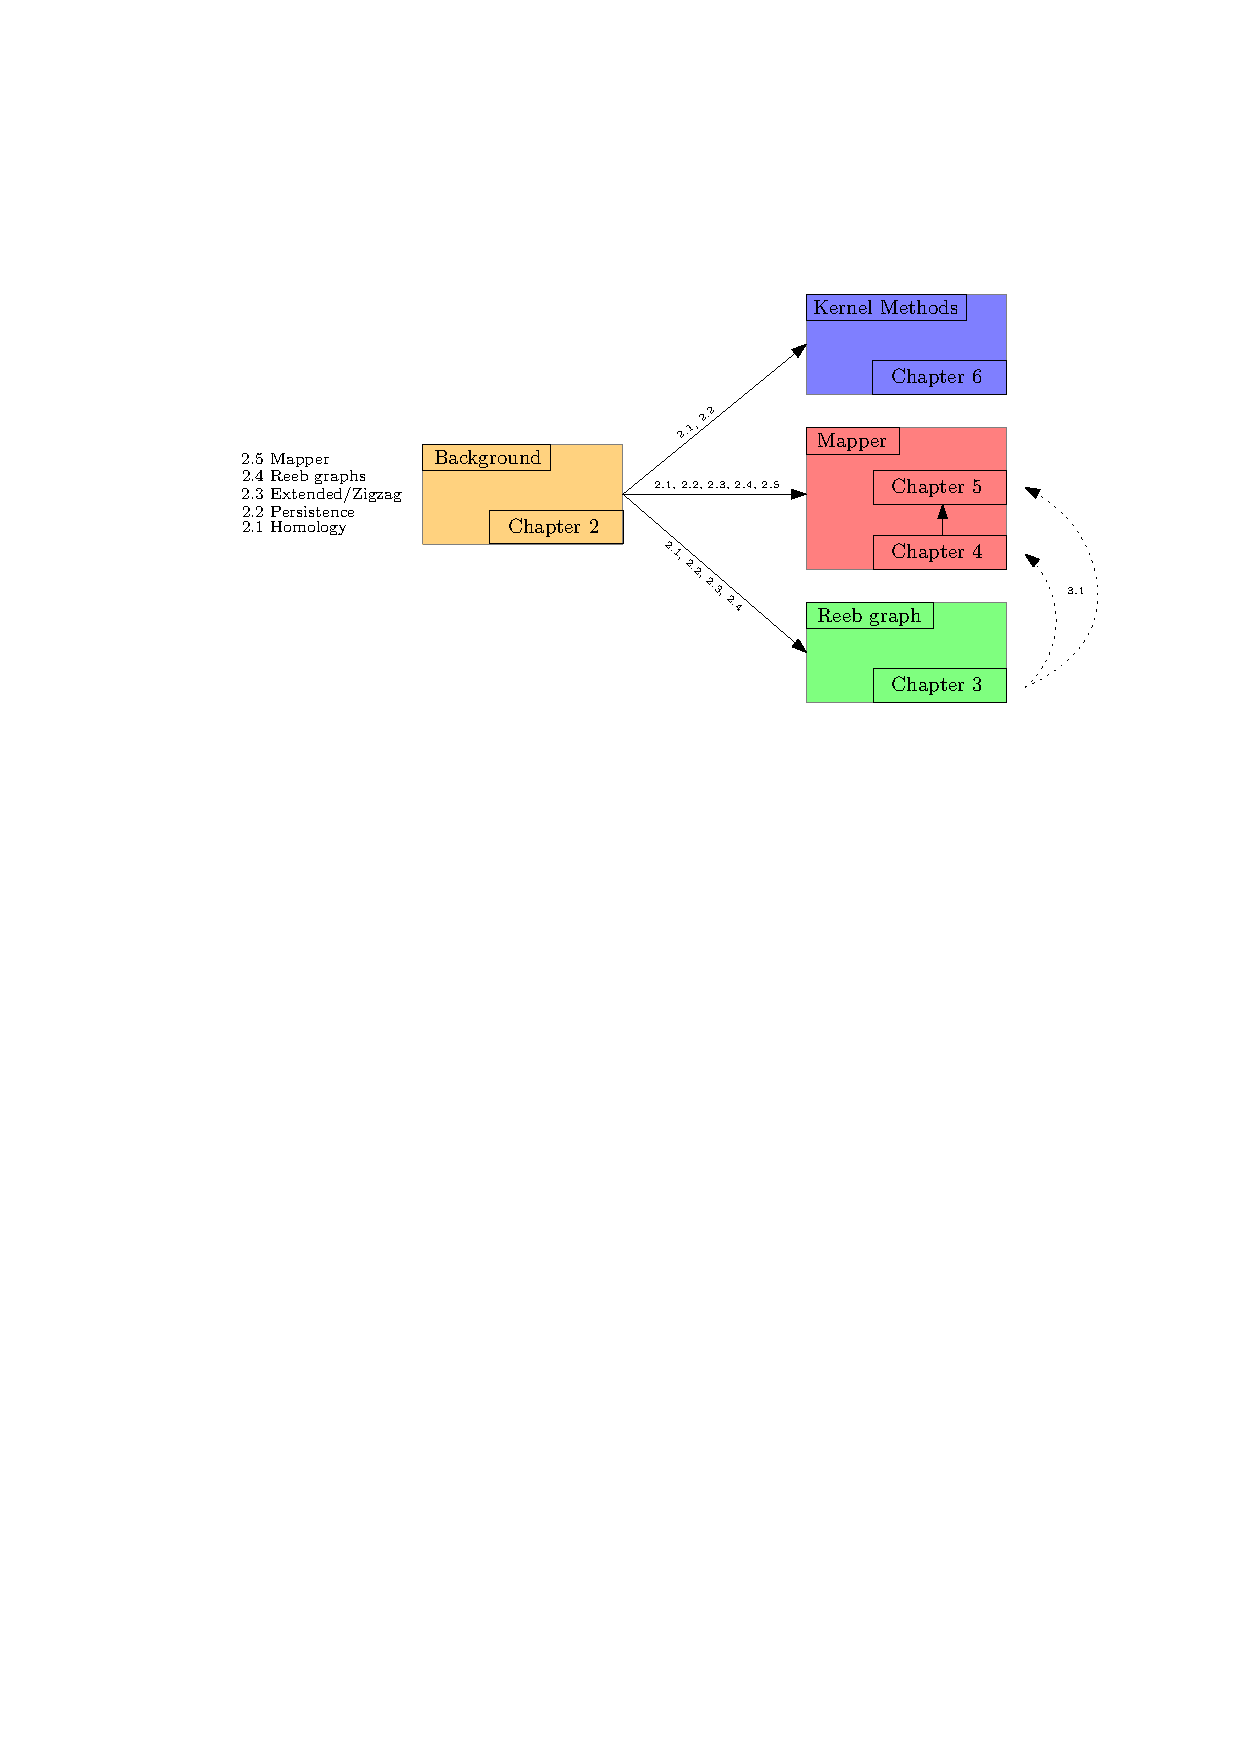
\includegraphics[width=0.95\textwidth]{figures/ThesisPlan}
\caption[Plan of the thesis]{\label{fig:thesis} Plain arrows indicate dependence between chapters, and dotted arrows indicate partial dependence, meaning 
that only a small, skippable part of the chapter depends on the other. 
%We also point out the background sections of 
%Chapter~\ref{chap:backgroundHomologyPersistence} which are required for each part.
}
\end{figure}


%Hence, the reader which is unfamiliar  
%In Chapter~\ref{chap:MapperStability}, we provide links between Mapper and Reeb graphs in the case of non discrete topological spaces.
%We also define a distance between Mapper from the one between Reeb graphs introduced in the previous chapter. We also show a stability theorem 
%for Mappers equipped with this distance.
%Chapter~\ref{chap:MapperStatistic} is a direct continuation of chapter~\ref{chap:MapperStability}.
%\end{itemize}



